% !TeX encoding = UTF-8
% Do not touch the below 70 lines
\documentclass[11pt, a4paper, onecolumn, oneside]{report}

\usepackage{mathptmx}
\usepackage[T1]{fontenc}
\usepackage[utf8]{inputenc}

\RequirePackage[top=3cm, bottom=1in, left=1in, right=1in]{geometry}
\linespread{1.3}

\usepackage{titlesec}
\usepackage{amsmath}
\usepackage{amssymb}
\usepackage{mathtools}
\usepackage{enumerate}
\usepackage{bbm}
\usepackage{algorithm}
\usepackage{algorithmic}
\usepackage{epsfig}
\usepackage{color}
\usepackage{graphicx}
\usepackage{caption}
\usepackage{subcaption}
\usepackage{cases}
\usepackage{url}
\usepackage{cite}
\usepackage{fancyhdr}
\usepackage{tocloft}
\usepackage{pdfpages}

\usepackage{acro}
\usepackage[notocbib]{apacite}
\usepackage{kotex}
\usepackage{microtype}
\usepackage{multirow}
\usepackage{rotating}
\usepackage{xurl}
\usepackage{lineno}
\usepackage{enumitem}
\setcounter{secnumdepth}{5}
\setcounter{tocdepth}{5}

\DeclareAcronym{ptb}
{
    short=PTB,
    long=Preterm birth
}

\DeclareAcronym{rrna}
{
    short=rRNA,
    long=Ribosomal RNA
}

\DeclareAcronym{ftb}
{
    short=FTB,
    long=Full-term birth
}

\DeclareAcronym{dat}
{
    short=DAT,
    long=Differentially abundant taxa
}

\DeclareAcronym{prom}
{
    short=PROM,
    long=Prelabor rupture of membrane
}

\DeclareAcronym{ga}
{
    short=GA,
    long=Gestational age
}

\DeclareAcronym{acc}
{
    short=ACC,
    long=Accuracy
}

\DeclareAcronym{ba}
{
    short=BA,
    long=Balanced accuracy
}

\DeclareAcronym{sen}
{
    short=SEN,
    long=Sensitivity
}

\DeclareAcronym{spe}
{
    short=SPE,
    long=specificity
}

\DeclareAcronym{pre}
{
    short=PRE,
    long=Precision
}

\DeclareAcronym{asv}
{
    short=ASV,
    long=Amplicon sequence variant
}

\DeclareAcronym{faithpd}
{
    short=Faith PD,
    long=Faith's phylogenetic diversity
}



\renewcommand\cftsecafterpnum{\vskip15pt}
\renewcommand\cftsubsecafterpnum{\vskip15pt}
\renewcommand\cftfigafterpnum{\vskip15pt}
\renewcommand{\thesection}{\arabic{section}}
\renewcommand{\thesubsection}{\arabic{section}.\arabic{subsection}}
\renewcommand{\thesubsubsection}{\arabic{section}.\arabic{subsection}.\arabic{subsubsection}}
\renewcommand{\contentsname}{\hfill\bfseries\Large Contents\hfill}
\renewcommand{\listfigurename}{\hfill\bfseries\Large List of Figures\hfill}
\renewcommand{\listtablename}{\hfill\bfseries\Large List of Tables\hfill}
\renewcommand{\thefigure}{\arabic{figure}}
\newcommand{\qed}{\hfill\blacksquare}
\renewcommand{\bibname}{\hfill\bfseries\Large References \hfill\hfill}
\renewcommand{\abstractname}{\bfseries\Large Abstract \hfill\hfill}

\newcounter{lemma}
\newcounter{proposition}
\newcounter{theorem}
\newtheorem{lemma}{\bf Lemma}
\newtheorem{proposition}{\bf Proposition}
\newtheorem{theorem}{\bf Theorem}
\newtheorem{proof}{\bf Proof}

\newcommand{\HIGH}[1]{{\textcolor{blue}{#1}}}
%\renewcommand{\baselinestretch}{1.5}

\DeclareMathOperator*{\argmax}{arg\,max}

\fancyhf{}
\renewcommand{\headrulewidth}{0pt}
\cfoot{\thepage}
\pagestyle{fancy}
%\pagenumbering{gobble}

% Do not touch the above 70 lines

\begin{document}
    \linenumbers
% Front cover
    \begin{center}
    \LARGE Doctoral Thesis

    \vspace{3cm}
    \huge \input{Documents/Title.txt}

    \vfill

    \LARGE \input{Documents/Name.txt}

    \vspace{2cm}

    \LARGE \input{Documents/Department.txt}

    \vspace{2cm}

    \LARGE \input{Documents/UNIST.txt}
    \vspace{2cm}

    \LARGE \the\year{}

    \end{center}
    \thispagestyle{empty}
    \clearpage

% Title page
    \begin{center}
    \hbox{ }

    \hbox{ }

    \huge \input{Documents/Title.txt}

    \vspace{5cm}

    \LARGE \input{Documents/Name.txt}

    \vspace{6cm}

    \LARGE \input{Documents/Department.txt}

    \vspace{2cm}

    \LARGE \input{Documents/UNIST.txt}

    \end{center}
    \thispagestyle{empty}
    \clearpage

% Thesis approval
% Add the approval doc signed by your advisor in a PDF file
% Put your pdf with the filename below, and uncomment it.
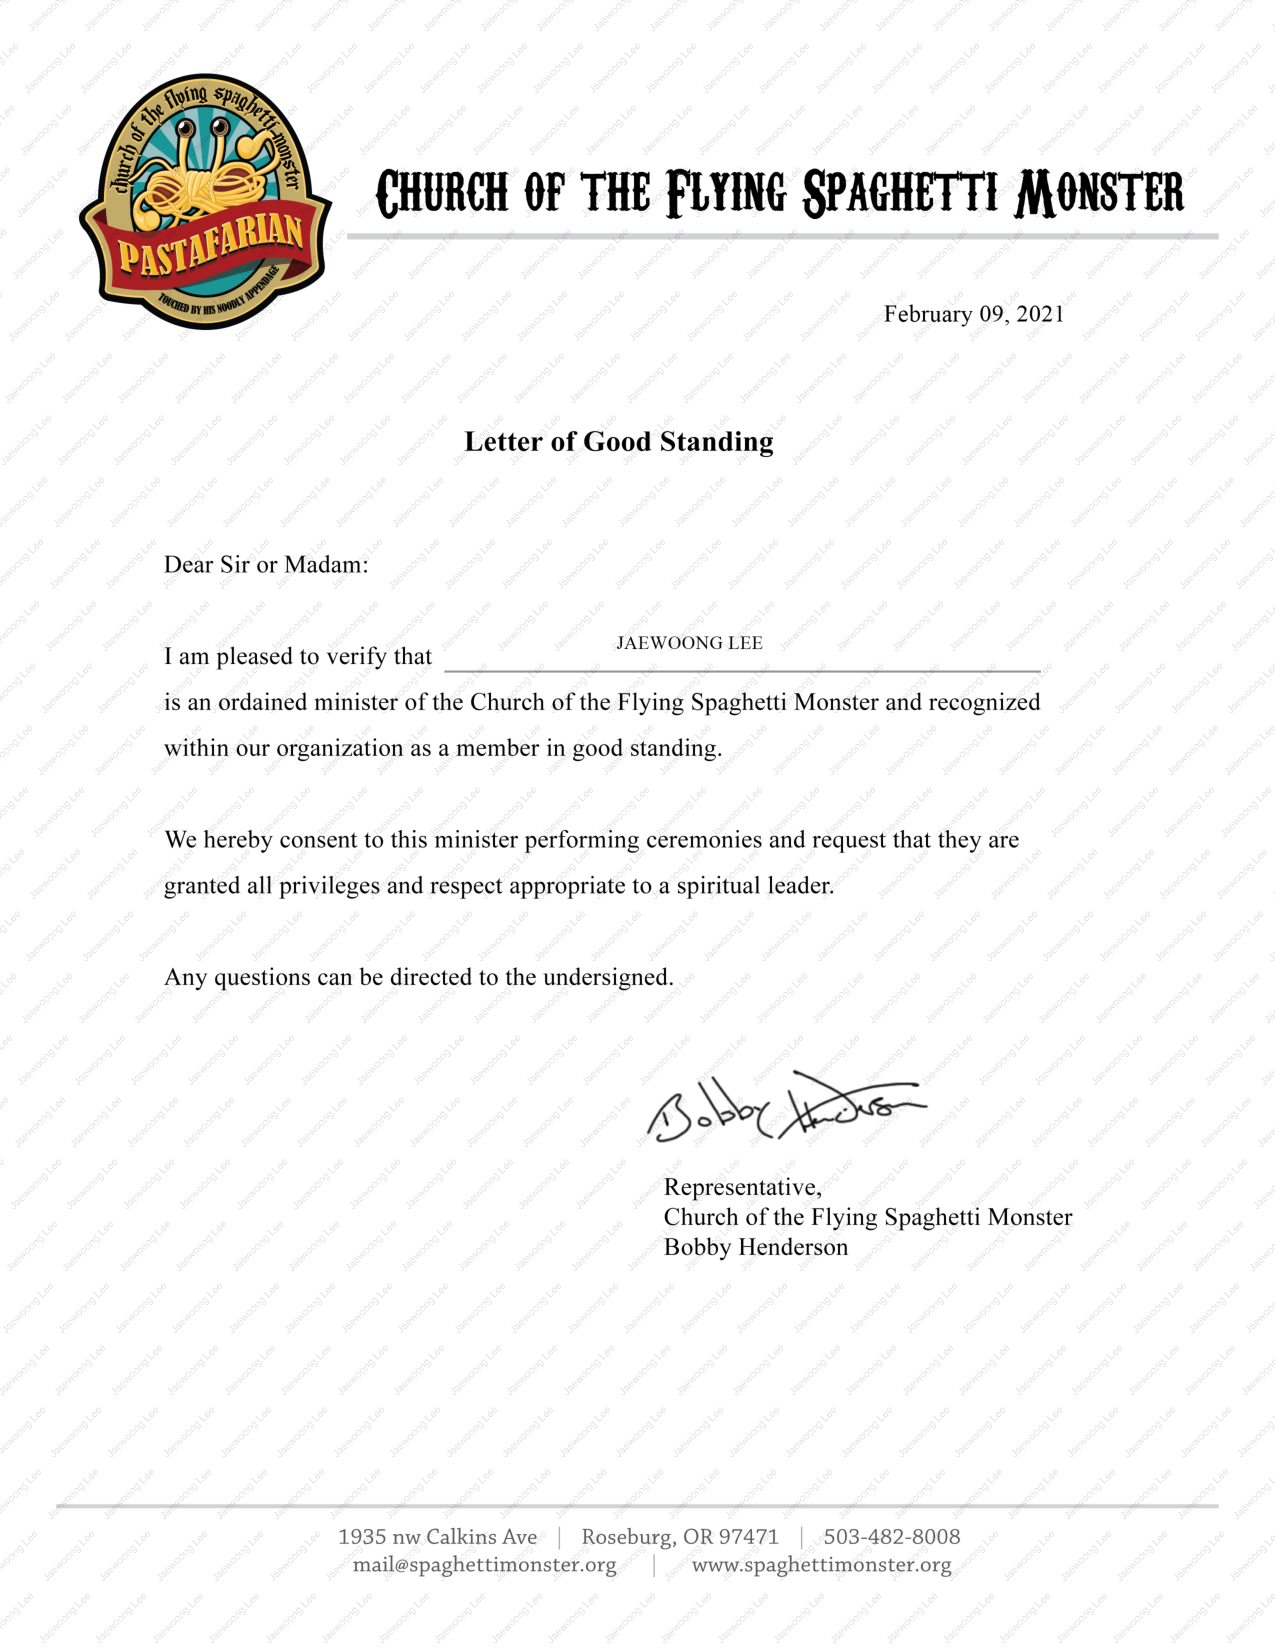
\includepdf[fitpaper= true, pages=-]{Documents/example.pdf}

% [Confirmation of thesis approval]
% add the certificate signed by your committee in a PDF file
% Put your pdf with the filename below, and uncomment it.
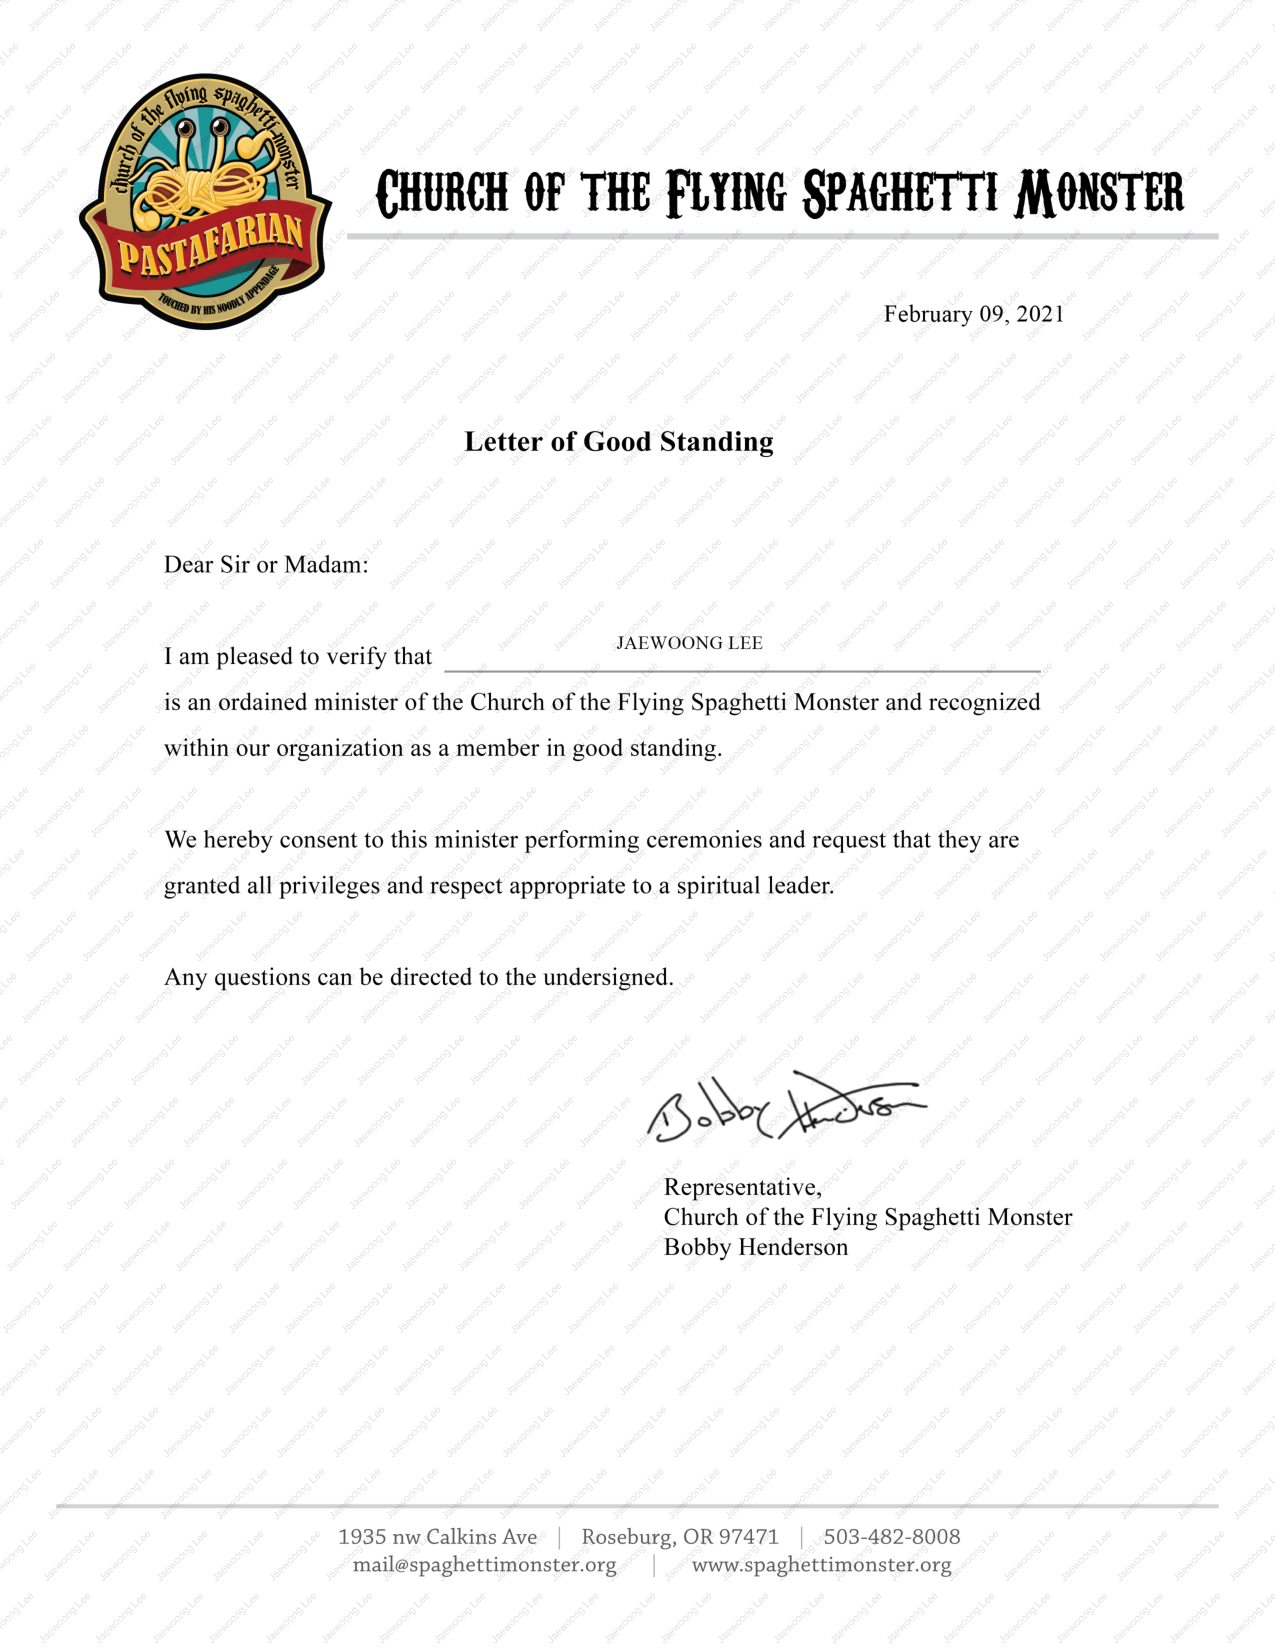
\includepdf[fitpaper= true, pages=-]{Documents/example.pdf}

% Abstract
    \begin{abstract}
        (Microbiome)

        (PTB) Section \ref{section:PTB} introduces...

        (Periodontitis) Section \ref{section:Periodontitis} describes...

        (Colon) Setion \ref{section:CRC}...

        (Conclusion)

        \vfill
        \noindent\rule{\linewidth}{0.4pt}
        \textbf{This doctoral dissertation is an addition based on the following papers that the author has already published}:
        \begin{itemize}
            \item \input{Documents/PTB.txt} \nocite{PTB-JW-1}
        \end{itemize}
    \end{abstract}
    \clearpage

% Do not touch the below 20 lines
\hbox{ }
\thispagestyle{empty}
\clearpage

%%% Table of Contents
\pagenumbering{roman}
\tableofcontents{}
%\thispagestyle{empty}
\vfill
\clearpage

%%% List of Figures
\listoffigures{}
%\thispagestyle{empty}
\clearpage

%%% List of Tables
\listoftables{}
%\thispagestyle{empty}
\clearpage

%%% reset page numbering
%  Do not touch the above 20 lines

    \section*{\centering List of Abbreviations}
        \printacronyms[display=all, heading=none]
    \newpage

    \pagenumbering{arabic}
    \setcounter{page}{1}
    \section{Introduction}
        The microbiome refers to the complex community of microorganisms, including bacteria, viruses, fungi, and other microbes, that inhabit various environment within living organisms \cite{microbiome-1, microbiome-3}. In humans, the microbiome plays a crucial role in maintaining health \cite{microbiome-2}, influencing processes such as digestion \cite{microbiome-digestion-1}, immune response \cite{microbiome-immune-1, microbiome-immune-2, microbiome-immune-3}, and even mental health \cite{microbiome-mental-1, microbiome-mental-2, microbiome-mental-3}. These microbial communities are not static nor constant, but rather dynamic ecosystem that interacts with their host and respond to environmental changes. Recent studies have revealed that imbalances in the microbiome, known as dysbiosis, can contribute to a wide range of diseases, including obesity \cite{microbiome-obesity-1, microbiome-obesity-2, microbiome-obesity-3}, diabetes \cite{microbiome-diabetes-1, microbiome-diabetes-2, microbiome-diabetes-3}, infections \cite{microbiome-infection-1, microbiome-infection-2}, inflammatory conditions \cite{microbiome-inflammation-1, microbiome-inflammation-2, microbiome-inflammation-3}, and cancers \cite{microbiome-cancer-1, microbiome-cancer-2, microbiome-cancer-3, microbiome-cancer-4}. Thus, understanding the composition of the human microbiomes is essential for developing new therapeutic approaches that target these microbial populations to promote health and prevent diseases.

        The microbiome participates a crucial role in overall health, influencing not only digestion and immune function but also systemic and neurological processes through the brain-gut axis \cite{brain-gut-1, brain-gut-2, brain-gut-3}. The gut microbiota interact with the host through metabolic byproducts, immune signaling, and the production of neurotransmitters, \textit{e.g.} serotonin and dopamine, which are essential for brain function and cognition. Disruptions in microbial composition, known as dysbiosis, have been linked to various diseases, including inflammatory vowel disease \cite{dysbiosis-inflammatory-1, dysbiosis-inflammatory-2}, obesity \cite{dysbiosis-obesity-1, dysbiosis-obesity-2, dysbiosis-obesity-3}, diabetes \cite{dysbiosis-diabetes-1, dysbiosis-diabetes-2, dysbiosis-diabetes-3}, and cardiovascular diseases \cite{dysbiosis-cardio-2, dysbiosis-cardio-3}. Furthermore, the brain-gut axis, a bidirectional communication system between the gut microbiome composition and the central nervous system, has been implicated in mental disorders, \textit{e.g.} anxiety disorder, depressive disorder, and neurodegenerative diseases. Emerging evidence suggested that alterations in the host microbiome can influence mood, cognitive function, and even behavior through immune modulation, vagus nerve signaling, and microbial metabolites. These findings highlight the microbiome as a critical factor in maintaining host health and suggest that targeted interventions, namely probiotics, antibiotics, dietary modification, and microbiome-based therapies, may hold promise for improving both physical and metal comfort. Hence, understanding the microbial effects could lead to novel therapeutic strategies for a wide range of health conditions.

        16S ribosomal RNA (rRNA) gene sequencing is one of the most extensively applied methods for characterizing microbial communities by targeting the conserved 16S rRNA gene, which contains both highly conserved and variable regions in bacteria \cite{16S-1, 16S-2}. The conserved regions enable universal primer binding, while the variable regions provide the specificity needed to differentiate microbial taxa. Among these regions, the V3-V4 region is frequently selected for sequencing due to its balance between phylogenetic resolution and sequencing efficiency \cite{16S-3, 16S-4}. Therefore, the V3-V4 region offers sufficient variability to classify a wide range of bacteria taxa while maintaining compatibility with widely used sequencing platforms.

        On the other hand, PathSeq is a computational pipeline designed for the identification and analysis of microbial sequences within short-read human sequencing data, such as next-generation sequencing \cite{PathSeq-1, PathSeq-2}. PathSeq's scalable and effective processing of massive amounts of sequencing data allows large-scale microbial profiling possible. PathSeq workflow consists of two main phases: a subtractive phase and an analytic phase. The subtractive phase is removing human-derived reads by aligning them to a human reference genome; and, the analytic phase is mapping remaining reads to microbial reference databases, not only bacterial reference genome, but also archaeal, fungal, and viral reference genomes. This approach allows for the comprehensive detection of microbiome compositions, without a requirement for targeted amplification. PathSeq presents a more comprehensive and objective evaluation of microbiome compositions than conventional microbiome profiling techniques including 16S rRNA gene sequencing, capturing an assortment of microbial species beyond bacteria. Therefore, PathSeq is an effective instrument for metagenomic research, infectious disease study, and microbiome analysis in environmental and clinical contexts because of its capacity to operate with complex sequencing datasets \cite{PathSeq-analysis-1, PathSeq-analysis-2, PathSeq-analysis-3}.

        Diversity indices are essential techniques for evaluating the complexity and variety of microbial communities,in ecological and microbiological research \cite{Diversity-1, Diversity-2}. Alpha-diversity index attributes to the heterogeneity within a specific community, obtaining the number of different taxa and the distribution of taxa among the individuals, \textit{i.e.}, richness and evenness. On the other hand, beta-diversity index measures the variations in microbiome compositions between the individuals, highlighting differences among the microbiome compositions of the study participants \cite{Diversity-3}. Altogether, by providing a thorough understanding of microbiome compositions, diversity indices, \textit{e.g.} alpha-diversity and beta-diversity, allow us to investigate factors that affecting community variability and structure.

        Differentially abundant taxa (DAT) detection is a key analytical approach in microbiome study to identify microbial taxa that significantly differ in abundance between distinct study participant groups. This DAT detection method is particularly valuable for understanding how microbial communities vary across different conditions, such as disease states, environmental factors, and/or experimental treatments. Various statistical and computational techniques, \textit{e.g.} LEfSe \cite{LEfSe-1}, DESeq2 \cite{DESeq2-1}, ANCOM \cite{ANCOM-1}, and ANCOM-BC \cite{ANCOM-BC-1, ANCOM-BC-2}, are commonly used to assess differential abundance while accounting for compositional and sparsity-related challenges in microbiome composition data \cite{DAT-1, DAT-2}. Thus, identifying DAT can provide insights into microbial biomarkers associated with specific health conditions or disease statuses, enabling potential applications in diagnostics and therapeutics. However, due to the nature of microbiome composition data and the influence of sequencing depth, appropriate normalization and statistically adjustments are necessary to ensure reliable and stable detection of differentially abundant microbes \cite{DAT-3, DAT-4}. Integrating DAT detection analysis with functional profiling further enhances our understanding of the biological significance of microbial shifts or dysbiosis. As microbiome research advances, improving methodologies for DAT selection remains essential for uncovering meaningful microbial association and their potential roles in human diseases.

        Classification is one of the supervised machine learning techniques used to categorized data into predefined classes based on features within the data \cite{classification-1, classification-2}. In other words, the method learns the relationship between input features and their corresponding output classes through the process of training a classification model using labeled data. Classification models are essential for advising choices in a wide range of applications, including medical diagnostics \cite{classification-analysis-1}. Thus, researchers could uncover sophisticated connections in input features and corresponding classes and produce reliable prediction by utilizing machine learning classification.

        Random forest classification is one of the ensemble machine learning methods that constructs several decision trees during training and aggregates their results to provide classification predictions \cite{RF-1}. A portion of the features and classes--known as bootstrapping \cite{RF-2, RF-3, RF-4} and feature bagging \cite{RF-5, RF-6, RF-7}--are utilized to construct each tree in the forest. The majority vote from each tree determines the final classification, which lowers the possibility of overfitting in comparison to a single decision tree. Furthermore, random forest classifier offers several advantages, including its robustness to outliers and its ability to calculate the feature importance.

        Evaluating the performance of a machine learning classification model is essential to ensure its reliability and effectiveness in real-world solutions and applications \cite{classification-evaluation-1, classification-evaluation-5, classification-evaluation-6}. A confusion matrix is a tabular representation of predictions of classification, showing the counts of true positives (TP), true negatives (TN), false positives (FP), and false negatives (FN) (Table \ref{tab:confusion}). From this matrix, evaluations can be derived: accuracy (ACC; Equation \ref{eq:ACC}), balanced accuracy (BA; Equation \ref{eq:BA}), F1 score (F1; Equation \ref{eq:F1}), sensitivity (SEN; Equation \ref{eq:SEN}), specificity (SPE; Equation \ref{eq:SPE}), and precision (PRE; Equation \ref{eq:PRE}). These metrics are in $[0, 1]$ range and high metrics are good metrics. The confusion matrix also helps in identifying specific types of errors, such as a tendency to produce false positive or false negatives, offering valuable insights for improving the classification model. By combining the confusion matrix with other evaluation metrics, researchers can comprehensively assess the classification metrics and refine it for real-world solutions and applications.

        The receiver-operating characteristics (ROC) curve is a graphical representation used to evaluate the performance of a classification model by plotting the sensitivity against (1-specificity) at multiple threshold setting \cite{classification-evaluation-2, classification-evaluation-3, classification-evaluation-4}. The ROC curve illustrates the trade-off between detecting true positives while minimizing false positives, suggesting determining the optimal decision threshold for classification. A key metric derived from the ROC curve is the area-under-curve (AUC), which quantifies overall ability of the classification model to discriminate between positive and negative predictions. An AUC value of 0.5 indicates a model performing no better than random chance, while value closer to 1.0 suggests high predictive accuracy. Thus, by analyzing the AUC value of the ROC curve, researchers can compare different models and select the better classification model that offers the best balance between sensitivity and specificity for a given application.

        This dissertation present a comprehensive, multi-disease human microbiome analysis, bridging the association between preterm birth (PTB) (Section \ref{section:PTB}), periodontitis (Section \ref{section:Periodontitis}), and colorectal cancer (CRC) (Section \ref{section:CRC}) through a unified metagenomic approach. While previous studies have examined the role and characteristics of human microbiome in these diseases individually, this dissertation uniquely integrates human microbiome-driven insights across these diseases to identify shared and disease-specific microbial signatures. By applying high-throughput metagenomic sequencing, microbial diversity analysis, and advanced bioinformatics techniques, this dissertation aims to uncover novel microbiome-based biomarkers and mechanistic insights into how microbial communities influence these conditions. These findings contribute to a broader understanding of microbiome-mediated disease interactions and pave the way for personalized medicine strategies, including microbiome-targeted diagnostics and therapeutics.

        \begin{table}[p]
            \centering
            \caption{Confusion matrix}
            \label{tab:confusion}
            \begin{tabular}{cc|cc}
 &  & \multicolumn{2}{c}{Predicted} \\ \cline{3-4} 
 &  & Positive & Negative \\ \hline
\multicolumn{1}{l|}{\multirow{2}{*}{Actual}} & Positive & True positive (TP) & False negative (FN) \\
\multicolumn{1}{l|}{} & Negative & False positive (FP) & True negative (TN)
\end{tabular}

        \end{table}
        \clearpage

        \begin{equation}
            \textrm{ACC} = \frac{\textrm{TP} + \textrm{TN}}{\textrm{TP} + \textrm{FN} + \textrm{FP} + \textrm{TN}}
            \label{eq:ACC}
        \end{equation}
        \begin{equation}
            \textrm{BA} = \frac{1}{2} \times (\frac{\textrm{TP}}{\textrm{TP} + \textrm{FP}} + \frac{\textrm{TN}}{\textrm{TN} + \textrm{FN}})
            \label{eq:BA}
        \end{equation}
        \begin{equation}
            \textrm{F1} = \frac{2 \times \textrm{TP}}{2 \times \textrm{TP} + \textrm{FP} + \textrm{FN}}
            \label{eq:F1}
        \end{equation}
        \begin{equation}
            \textrm{SEN} = \frac{\textrm{TP}}{\textrm{TP} + \textrm{FP}}
            \label{eq:SEN}
        \end{equation}
        \begin{equation}
            \textrm{SPE} = \frac{\textrm{TN}}{\textrm{TN} + \textrm{FN}}
            \label{eq:SPE}
        \end{equation}
        \begin{equation}
            \textrm{PRE} = \frac{\textrm{TP}}{\textrm{TP} + \textrm{FP}}
            \label{eq:PRE}
        \end{equation}
        \clearpage
    \newpage

    \section{Predicting preterm birth using random forest classifier in salivary microbiome}
        \label{section:PTB}

        \textbf{This section includes the published contents}: \\
        \input{Documents/PTB.txt} \nocite{PTB-JW-1}

        \subsection{Introduction}
            Preterm birth (PTB), characterized by the delivery of neonates prior to 37 weeks of gestation, is one of the major cause to neonatal mortality and morbidity \cite{PTB-rate-1}. Multiple pregnancies including twins, short cervical length, and infection on genitourinary tract are known risk factor for PTB \cite{PTB-cause-1}. Nevertheless, the extent to which these aspects affect birth outcomes is still up for debate. Henceforth, strategies to boost gestation and enhance delivery outcomes can be more conveniently implemented when pregnant women at high risk of PTB are identified early \cite{PTB-care-1}.

            Prediction models that can be utilized as a foundation for intervention methods still have an unacceptable amount of classification evaluations, including accuracy, sensitivity, and specificity, despite a great awareness of the risk factors that trigger PTB \cite{PTB-prediction-1}. Several attempts have been made to predict PTB through integrating data such as human microbiome composition, inflammatory markers, and prior clinical data with predictive machine learning methods \cite{PTB-prediction-2}. Because it is affordable and straightforward to use, fetal fibronectin is commonly used in medical applications. However, with a sensitivity of only 56\% that merely similar to random prediction, it has a low classification evaluation \cite{PTB-prediction-3}. Due to the difficulty and imprecision of the method in general, as well as the requirement for a qualified specialist cervical length measuring is also restricted \cite{PTB-prediction-4}.

            Preterm prelabor rupture of membranes (PROM) brought on by gestational inflammation and infection contribute to about 70\% of PTB cases \cite{PTB-prediction-5}. Nevertheless, as antibiotics and anti-inflammatory therapeutic strategies were ineffective to decrease PTB occurrence rates, the pathology of PTB has not been entirely elucidated by inflammatory and infectious pathways \cite{PTB-mechanism-1}. Recent researches on maternal microbiomes were beginning to examine unidentified connections of PTB as a consequence of developmental processes in molecular biological technology \cite{PTB-mechanism-2}.

            However, as anti-inflammatory and antibiotic therapies were insufficient to lower PTB occurrence rates, infectious and inflammatory processes are insufficient to exhaustively clarify the pathogenesis and pathophysiology of PTB. It has been hypothesized that the microbiota linked to PTB originate from either a hematogenous pathway or the female genitourinary tract increasing through the vagina and/or cervix \cite{PTB-mechanism-3}. Vaginal microbiome compositions have been found in women who eventually acquire PTB, and recent studies have tried to predict PTB risk using cervico-vaginal fluid \cite{PTB-mechanism-4}. Even though previous investigation have confirmed the potential relationships between the vaginal microbiome compositions and PTB, these studies are only able to clarify an upward trajectory.

            Multiple unfavorable birth outcomes, including PROM and PTB, have been linked to periodontitis as an independence risk factor, according to numerous epidemiological researches \cite{PTB-mechanism-5}. It is expected that the oral microbiome will be able to explain additional hematogenous pathways in light of these precedents; however, the oral microbiome composition of fetuses is limited understood.

            Hence, in order to identify the salivary microbiome linked to PTB and to establish a machine learning prediction model of PTB determined by oral microbiome compositions, this study examined the salivary microbiome compositions of PTB study participants with a full-term birth (FTB) study participants.
        \newpage

        \subsection{Materials and methods}
            \subsubsection{Study design and study participants}
                Between 2019 and 2021, singleton pregnant women who received treatment to Jeonbuk National University Hospital for childbirth were the participants of this study. This study was conducted according to the Declaration of Helsinki \cite{Helsinki-1}. The Institutional Review Board authorized this study (IRB file No. 2019-01-024). Participants who were admitted for elective cesarean sections (C-sections) or induction births, as well as those who had written informed consent obtained with premature labor or PROM, were eligible.

            \subsubsection{Clinical data collection and grouping}
                Questionnaires and electronic medical records were implemented to gather information on both previous and current pregnancy outcomes. The following clinical data were analyzed:
                \begin{itemize}[noitemsep, nolistsep]
                    \item maternal age at delivery
                    \item diabetes mellitus
                    \item hypertension
                    \item overweight and obesity
                    \item C-section
                    \item history PROM or PTB
                    \item gestational week on delivery
                    \item birth weight
                    \item sex
                \end{itemize}

            \subsubsection{Salivary microbiome sample collection}
                Salivary microbiome samples were collected 24 hours before to delivery using mouthwash. The standard methods of sterilizing were performed. Medical experts oversaw each stage of the sample collecting procedure. Participants received instruction not to eat, drink, or brush their teeth for 30 minutes before sampling salivary microbiome. Saliva samples were gathered by washing the mouth for 30 seconds with 12 mL of a mouthwash solution (E-zen Gargle, JN Pharm, Pyeongtaek, Gyeonggi, Korea). The samples were tagged with the anonymous ID for each participant and kept at 4 \textcelsius until they underwent further processing. Genomic DNA was extracted using an ExgeneTM Clinic SV kit (GeneAll Biotechnology, Seoul, Korea) following with the manufacturer instructions and store at -20 \textcelsius.

            \subsubsection{16s rRNA gene sequencing}
                Salivary microbiome samples were transported to the \input{Documents/Department.txt} of the \input{Documents/UNIST.txt}. 16S rRNA sequencing was then carried out using a commissioned Illumina MiSeq Reagent Kit v3 (Illumina, San Diego, CA, USA). Library methods were utilized to amplify the V3-V4 areas. 300 base-pair paired-end reads were produced by sequencing the pooled library using a v3 $\times$600 cycle chemistry after the samples had been diluted to a final concentration of 6 pM with a 20\% PhiX control.

            \subsubsection{Bioinformatics analysis}
                The independent $t$-test was utilized to evaluate the differences of continuous values between from the PTB participants than the FTB participants; $\chi$-square test was applied to decide statistical differences of categorical values. Clinical measurement comparisons were conducted using SPSS (version 20.0) \cite{SPSS-1}. At $p < 0.05$, statistical significance was taken into consideration.

                QIIME2 (version 2022.2) was implemented to import 16S rRNA gene sequences from salivary microbiome samples of study participants for additional bioinformatics processing \cite{QIIME2-1}. DADA2 was used to verify the qualities of raw sequences \cite{DADA2-1}. The remain sequences were clustered into amplicon sequence variants (ASVs). Diversity indices, namely Faith PD for alpha diversity index \cite{FaithPD-1} and Hamming distance for beta diversity index \cite{Hamming-1}, were calculated. MWU test \cite{MWW-1}, and PERMANOVA multivariate test were evaluated for measuring statistical significance \cite{PERMANOVA-1, PERMANOVA-2}.

                Taxonomic assignment were implemented with HOMD (version 15.22) \cite{HOMD-1}. Afterward, DESeq2 was implemented to identify differentially abundant taxa (DAT) that could distinguish between salivary microbiome from PTB and FTB participants \cite{DESeq2-1}. Taxa with $| \log _2 \textrm{FoldChange} | > 1$ and $p < 0.05$ were considered as statistically significant.

                The taxa for predicting PTB using salivary microbiome data were determined using a random forest classifier \cite{RF-1}. Through stratified $k$-fold cross-validation ($k=5$) that preserves the existence rate of PTB and FTB participants, consistency and trustworthy classification were ensured \cite{Kfold-1}.

            \subsubsection{Data and code availability}
                All sequences from the 59 study participants have been published to the Sequence Read Archives (project ID \texttt{PRJNA985119}): \url{https://dataview.ncbi.nlm.nih.gov/object/PRJNA985119}. Docker image that employed throughout this study is available in the DockerHub: \url{https://hub.docker.com/r/fumire/helixco_premature}. Every code used in this study can be found on GitHub: \url{https://github.com/CompbioLabUnist/Helixco_Premature}.
        \newpage

        \subsection{Results}
            \subsubsection{Overview of clinical information}
                In the beginning, 69 volunteer mothers were recruited for this study. However, due to insufficient clinical information or twin pregnancies, 10 participants were excluded from the study participants. Demographic and clinical information of the study participants are displayed in Table \ref{tab:PTB-clinical}. Because PROM is one of the leading factors of PTB, it was prevalent in the PTB group than the FTB group. Other maternal clinical factors did not significantly differ between the FTB and PTB groups. There were no cases in both groups that had a history of simultaneous periodontal disease or cigarette smoking.

            \subsubsection{Comparison of salivary microbiomes composition}
                The salivary microbiome composition was composed of 13953804 sequences from 59 study participants, with 102305.95$\pm$19095.60 and 64823.41$\pm$15841.65 (mean$\pm$SD) reads/sample before and following the quality-check stage, accordingly. There was not a significant distinction between the PTB and FTB groups with regard to on alpha diversity nor beta diversity metrics (Figure \ref{fig:PTB-diversity}).

                DESeq2 was used to select 32 DAT that distinguish between the PTB and FTB groups out of the 465 species that were examined \cite{DESeq2-1}: 26 FTB-enriched DAT and six PTB-enriched DAT. Seven PROM-related DAT were removed from these 32 PTB-related DAT to lessen the confounding effect of PROM (Figure \ref{fig:PTB-volcano}). Therefore, there were a total of 25 PTB-related DAT: 22 FTB-enriched DAT and three PTB-enriched DAT (Figure \ref{fig:PTB-DAT}).

                A significant negative correlation was found using Pearson correlation analysis between GW and differences between PTB-enriched DAT and FTB-enriched DAT ($r = \textrm{-}0.542$ and $p = 7.8\textrm{e-}6$; Figure \ref{fig:PTB-volcano}).

            \subsubsection{Random forest classification to predict PTB risk}
                To classify PTB according to DAT, random forest classifiers were constructed. The nine most significant DAT were used to obtain the best BA (0.765$\pm$0.071; Figure \ref{fig:PTB-ML}a). Moreover, random forest classification model determined each DAT's importance (Figure \ref{fig:PTB-ML}b). We conducted a validation procedure on nine twin pregnancies that were excluded in the initial study design in order to confirm the reliability and dependability of our random forest-based PTB prediction model (Figure \ref{fig:PTB-validation}). Comparable to the PTB prediction model on the 59 initial singleton study participants, the validation classification on PTB risk of these twin participants have an accuracy of 87.5\%.

            \begin{table}[p]
                \centering
                \caption[Standard clinical information of study participants]{\textbf{Standard clinical information of study participants}. \\
                    Continuous variable for independent $t$-test. Categorical variable for Pearson's $\chi$-square test. Continuous variable: mean$\pm$SD. Categorical vaiable: count (proprotion)}
                    \begin{tabular}{l|llr}
 & PTB (n=30) & FTB (n=29) & p \\ \hline
Maternal age (years) & 31.8$\pm$5.2 & 33.7$\pm$4.5 & 0.687 \\
C-section & 20 (66.7\%) & 24 (82.7\%) & 0.233 \\
Previous PTB history & 4 (13.3\%) & 1 (3.4\%) & 0.353 \\
PROM & 12 (40.0\%) & 1 (3.4\%) & 0.001 \\
Pre-pregnant overweight & 8 (26.7\%) & 7 (24.1\%) & 1.000 \\
Gestational weight gain (g) & 9.0$\pm$5.9 & 11.5$\pm$4.6 & 0.262 \\
Diabetes & 2 (6.7\%) & 2 (6.9\%) & 1.000 \\
Hypertension & 11 (36.7\%) & 4 (13.8\%) & 0.072 \\
Gestational age (weeks) & 32.5$\pm$3.4 & 38.3$\pm$1.1 & $\le$0.001 \\
Birth weight (g) & 1973.4$\pm$686.6 & 3283.4$\pm$402.7 & $\le$0.001 \\
Male & 14 (46.7\%) & 13 (44.8\%) & 1.000
\end{tabular}

                \label{tab:PTB-clinical}
            \end{table}
            \clearpage

            \begin{figure}[p]
                \centering
                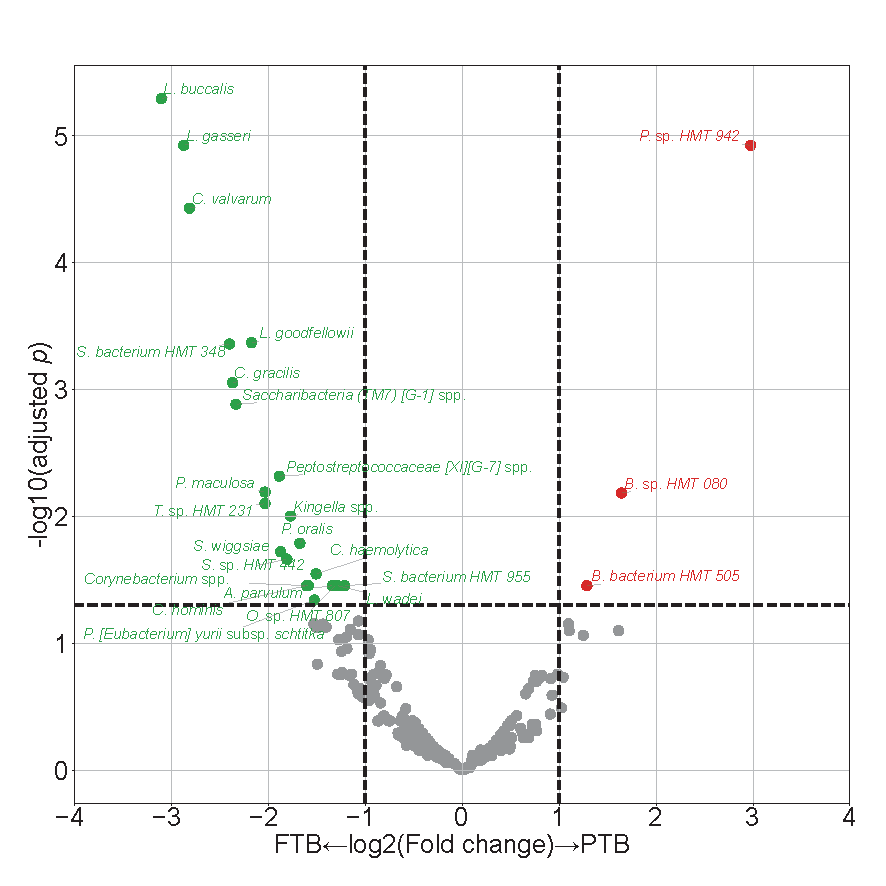
\includegraphics[width=\linewidth]{Figures/PTB/Fig1-DAT.pdf}
                \caption[DAT volcano plot]{\textbf{DAT volcano plot}. \\
                    Red dots represent PTB-enriched DAT, while green dots represent FTB-enriched DAT.}
                \label{fig:PTB-DAT}
            \end{figure}
            \clearpage

            \begin{figure}[p]
                \centering
                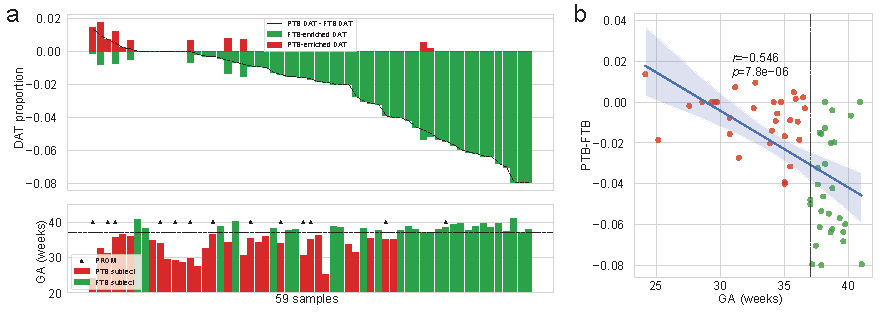
\includegraphics[width=\linewidth]{Figures/PTB/Fig2-Composition.pdf}
                \caption[Salivary microbiome compositions over DAT]{\textbf{Salivary microbiome compositions over DAT}. \\
                    \textbf{(a)} Frequencies of DAT of study subjects. The study participants are arranged in respect of $(\textrm{PTB-enriched DAT} - \textrm{FTB-enriched DAT})$. The study participants' GA is displayed in accordance with the upper panel's order (PTB: red bar, FTB: green bar. PROM: arrow head.) \textbf{(b)} Correlation plot with GA and $(\textrm{PTB-enriched DAT} - \textrm{FTB-enriched DAT})$. Strong negative correlation is found with Pearson correlation.}
                \label{fig:PTB-composition}
            \end{figure}
            \clearpage

            \begin{figure}[p]
                \centering
                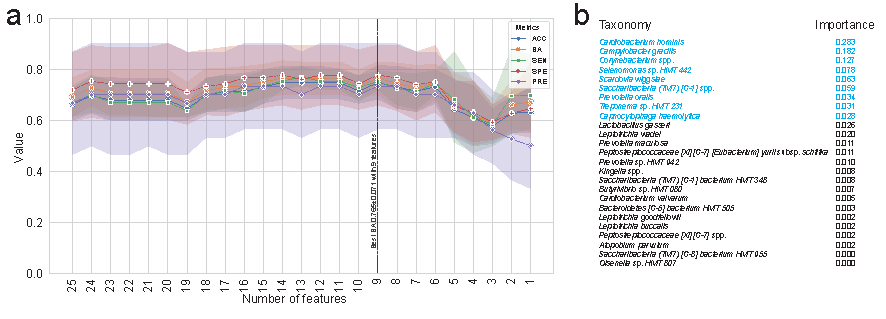
\includegraphics[width=\linewidth]{Figures/PTB/Fig3-ML.pdf}
                \caption[Random forest-based PTB prediction model]{\textbf{Random forest-based PTB prediction model}. \\
                    \textbf{(a)} Machine learning evaluations upon number of features (DAT). Random Forest classifier has the best BA (0.765$\pm$0.071; Mean$\pm$SD) with the nine most important DAT. \textbf{(b)} Importance of DAT.}
                \label{fig:PTB-ML}
            \end{figure}
            \clearpage

            \begin{figure}[p]
                \centering
                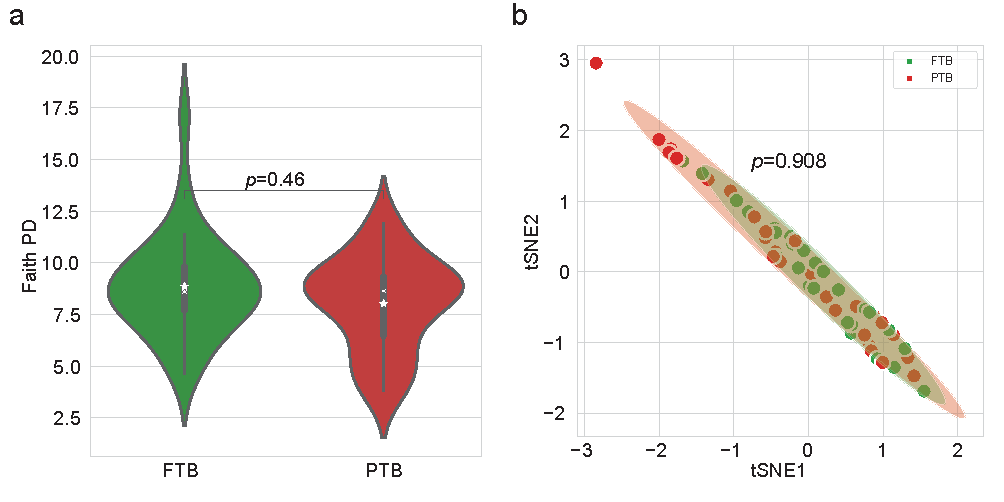
\includegraphics[width=\linewidth]{Figures/PTB/FigS1-Diversity.pdf}
                \caption[Diversity indices]{\textbf{Diversity indices}. \\
                    \textbf{(a)} Alpha diversity index (Faith PD). There is no statistically significant difference between the PTB and FTB group (MWU test $p=0.46$). \textbf{(b)} t-SNE plot with beta diversity index (Hamming distance). There is no statistically significant difference between the PTB and FTB group (PERMANOVA test $p=0.908$)}
                \label{fig:PTB-diversity}
            \end{figure}
            \clearpage

            \begin{figure}[p]
                \centering
                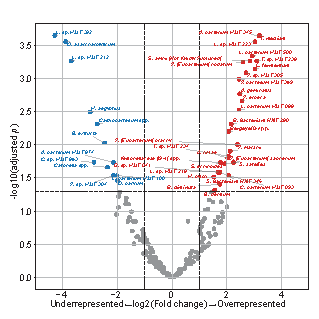
\includegraphics[width=\linewidth]{Figures/PTB/FigS2-PROM.pdf}
                \caption[PROM-related DAT]{\textbf{PROM-related DAT}. \\
                    Only seven of these 42 PROM-related DAT overlapped with PTB-related DAT (bold text). Blue dots represented PROM-underrepresented DAT, while red dots represented PROM-overrepresented DAT.}
                \label{fig:PTB-volcano}
            \end{figure}
            \clearpage

            \begin{figure}[p]
                \centering
                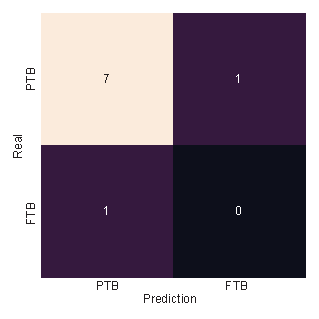
\includegraphics[width=\linewidth]{Figures/PTB/FigS3-validation}
                \caption[Validation of random forest-based PTB prediction model]{\textbf{Validation of random forest-based PTB prediction model}. \\
                    Nine twin pregnancies (eight PTB subjects and a FTB subject) that were excluded in the initial study subjects were subjected to a validation procedure. The random forest-based PTB prediction model shows 87.5\% accuracy, comparable to the PTB classification evaluations on the singleton study subjects (0.714$\pm$0.061. Mean$\pm$SD)}
                \label{fig:PTB-validation}
            \end{figure}
            \clearpage
        \newpage

        \subsection{Discussion}
            In this study, we employed salivary microbiome compositions to develop the random forest-based PTB prediction models to estimate PTB risks. Previous reports have indicated bidirectional associations between pregnancy outcomes and salivary microbiome compositions \cite{PTB-mechanism-3}. Nevertheless, the salivary microbiome composition is not yet elucidated. Salivary microbial dysbiosis, including gingival inflammation and periodontitis, have been connected to unfavorable pregnancy outcomes, such as PTB \cite{PTB-mechanism-6}. However, the techniques utilized in recent research that primarily focus on recognized infections have led to inconsistent outcomes.

            One of the most common salivary taxa that has been examined is \textit{Fusobacterium nucleatum} \cite{Fusobacterium-1, Fusobacterium-2, Fusobacterium-3}, that is a Gram-negative, anaerobic, and filamentous bacteria. \textit{Fusobacterium nucleatum} can be separated from not only the salivary microbiome but also the vaginal microbiome \cite{PTB-mechanism-7, PTB-mechanism-8}. In both animal and human investigation, \textit{Fusobacterium nucleatum} infection has been linke to risk of PTB \cite{Fusobacterium-4}. According to recent researches, the placenta women who give birth prematurely may include additional salivary microbiome dysbiosis, such as \textit{Bergeyella} spp. and \textit{Porphyromonas gingivalis} \cite{Porphyromonas-1, Porphyromonas-2}. Although \textit{Bergeyella} spp. were one of the PROM-overrepresented DAT (Figure \ref{fig:PTB-volcano}), it was excluded in the final 25 PTB-related DAT. Furthermore,  \textit{Porpyhromonas gingivalis} and \textit{Campylobacter gracilis} were pathogens of periodontitis in sub-gingival microbiome \cite{PTB-mechanism-9}. \textit{Lactobacillus gasseri} was also one of the FTB-enriched DAT (Figure \ref{fig:PTB-DAT}), and it is well established that early PTB risk can be reduced by \textit{Lactobacillus gasseri} in the vaginal microbiome \cite{PTB-mechanism-10, PTB-mechanism-11}.

            With DAT comprising 22 FTB-enriched DAT and three PTB-enriched DAT (Figure \ref{fig:PTB-DAT}), we discovered that the FTB study participants had the majority of the essential DAT that distinguished between the PTB and FTB groups. Thus, we hypothesize that the pathogenesis and pathophysiology of PTB may have been triggered by an absence of species with protective characteristics. The association between unfavorable pregnancy outcomes and a dysfunctional microbiome has been explained through two distinct processes. According to the first hypothesis, periodontal pathogens originating in the gingival biofilm might spread from the infected salivary microbiome over the placenta microbiome, invade the intra-amniotic fluid and fetal circulation, and then have a direct impact on the fetoplacental unit, leading to bacteremia \cite{Periodontitis-1}. Based on the second hypothesis, inflammatory mediators and endotoxins that generated by the sub-gingival inflammation and derived from dental plaque of periodontitis may spread throughout the body and reach the fetoplacental unit \cite{PTB-mechanism-12, PTB-mechanism-13}. Despite belonging to the same species, some subgroups of the salivary microbiome may influence pregnancy outcomes in both favorable and adverse manners. Following this line of argumentation, the salivary microbiome composition or their dysbiosis are more significant than the existence of particular bacteria.

            Notably, microbial alteration that take place throughout pregnancy may be expected results of a healthy pregnancy. Those pregnancy-related vulnerabilities to dental problem like periodontitis can be explained by three factors. Because of hormone-driven gingival hyper-reactivity to the salivary microbiome in the oral biofilm including sub-gingival biofilm, these conditions are prevalent in pregnant women. For insight at the relationship between the salivary microbiome compositions and PTB, further studies with pathway analysis are warranted.

            Our study confirmed that salivary microbiome composition could provide potential biomarkers for predicting pregnancy complications including PTB risks using random forest-based classification models, despite a limited number of study participants and a tiny validation sample size. Another limitation of our study was 16S rRNA sequencing. In other words, unlike the shotgun sequencing, 16S rRNA gene sequencing only focused on bacteria, not viruses nor fungi. We did not delve into other variables like nutrition status and socioeconomic statuses of study participants that might affect the salivary microbiome composition.

            Notwithstanding these limitations, this prospective examination showed the promise of the random forest-based PTB prediction models based on mouthwash-derived salivary microbiome composition. Before applying the methods developed in this study in a clinical context, more multi-center and extensive research is warranted to validate our findings.
        \newpage

    \section{Random forest prediction model for periodontitis statuses based on the salivary microbiomes}
        \label{section:Periodontitis}

        \subsection{Introduction}
            Saliva microbial dysbiosis brought on by the accumulation of plaque results in periodontitis, a chronic inflammatory disease of the tissue that surrounds the tooth \cite{Periodontitis-2}. Loss of periodontal attachment is a consequence of periodontitis, which may lead to irreversible bone loss and, eventually, permanent tooth loss if left untreated. A new classification criterion of periodontal diseases was created in 2018, about 20 years after the 1999 statements of the previous one \cite{Periodontitis-4}. Even with this evolution, radiographic and clinical markers of periodontitis progression remain the primary methods for diagnosing periodontitis \cite{Periodontitis-4}. Such tools, nevertheless, frequently demonstrate the prior damage from periodontitis rather than its present condition. Certain individuals have a higher risk of periodontitis, a higher chance of developing severe generalized periodontitis, and a worse response to common salivary bacteria control techniques utilized to prevent and treat periodontitis. As a result, the 2017 framework for diagnosing periodontitis additionally allows for the potential development of biomarkers to enhance diagnosis and treatment of periodontitis \cite{Periodontitis-5}. Instead of only depending on the progression of periodontitis, a new etiological indication based on the current state must be introduced in order to enable appropriate intervention through early detection of periodontitis. Thus, the current clinical diagnostic techniques that rely on periodontal probing can be uncomfortable for patients with periodontitis \cite{Periodontitis-6}.

            Due to the development of salivaomics, in this manner, the examination of saliva has emerged as a significant alternative to the conventional ways of identifying periodontitis \cite{Periodontitis-diagnosis-1, Periodontitis-diagnosis-2}. Given that saliva sampling is non-invasive, painless, and accessible to non-specialists, it may be a valuable instrument for diagnosing periodontitis \cite{Periodontitis-diagnosis-3}. Furthermore, much research has suggested that periodontitis could be a trigger in the development and exacerbation of metabolic syndrome \cite{Periodontitis-metabolic-1, Periodontitis-metabolic-2}. Consequently, alteration in these levels of salivary microbiome markers may serve as high effective diagnostic, prognostic, and therapeutic indicators for periodontitis and other systemic diseases \cite{Periodontitis-diagnosis-4, Periodontitis-diagnosis-5}. The pathogenesis of periodontitis typically comprises qualitative as well as quantitative alterations in the salivary microbial community, despite that it is a complex disease impacted by a number of contributing factors including age, smoking status, stress, and nourishment \cite{Periodontitis-7, Periodontitis-8}. Depending on the severity of periodontitis, the salivary microbial community's diversity and characteristics vary \cite{Periodontitis-7}, indicating that a new etiological diagnostic standards might be microbial community profiling based on clinical diagnostic criteria. As a consequence, salivary microbiome compositions have been characterized in numerous research in connection with periodontitis. High-throughput sequencing, including 16S rRNA gene sequencing, has recently used in multiple studies to identify variations in the bacterial composition of sub-gingival plaque collections from periodontal healthy individuals and patients with periodontitis \cite{Periodontitis-9, Periodontitis-10, Periodontitis-11}. This realization has rendered clear that alterations in the salivary microbial community--especially, shifts to dysbiosis--are significant contributors to the pathogenesis and development of periodontitis \cite{Periodontitis-12}. Yet most of these research either focused only on the microbiome alterations in sub-gingival plaque collection, comprised a limited number of periodontitis study participants, or did not account for the impact of multiple severities of periodontitis.

            For the objective of diagnosing periodontitis, previous research has developed machine learning-based prediction models based on oral microbiome compositions, such as the sub-gingival microbial dysbiosis index \cite{Periodontitis-diagnosis-6, Periodontitis-diagnosis-7}, which have demonstrated good diagnostic evaluation and could be applied to individual saliva collection. Despite offering valuable details, these indicators are frequently restricted by their limited emphasis on classifying the multiple severities of periodontitis. Furthermore, many of these machine learning models currently in practice are trained solely upon the existence of periodontitis rather than on the multiple severities of periodontitis.

            Recently, we employed multiplex quantitative-PCR and machine learning-based classification model to predict the severity of periodontitis based on the amount of nine pathogens of periodontitis from saliva collections \cite{Periodontitis-diagnosis-8}. On the other hand, the fact that we focused merely at nine pathogens for periodontitis and neglected the variety bacterial species associated to the various severities of periodontitis constrained the breadth of our investigation. By developing a machine learning model that could classify multiple severities of periodontitis based on the salivary microbiome composition, this study aims to fill these knowledge gaps and produce more accurate and therapeutically useful guidance to evaluate progression of periodontitis. Hence, in order to examine the salivary microbiome composition of both healthy controls and patients with periodontitis in multiple stages, we applied 16S rRNA gene sequencing. Furthermore, employing the 2018 classification criteria, we sought to find biomarkers (species) for the precise prediction of periodontitis severities \cite{Periodontitis-4, Periodontitis-13}.
        \newpage

        \subsection{Materials and methods}
            \subsubsection{Study participants enrollment}
                Between 2018-08 and 2019-03, 250 study participants--100 healthy controls, 50 patients with stage I periodontitis, 50 patients with stage II periodontitis, and 50 patients with stage III periodontitis--visited visited the Department of Periodontics at Pusan National University Dental Hospital. The Institutional Review Board of the Pusan National University Dental Hospital accepted this study protocol and design (IRB No. PNUDH-2016-019). Every study participants provided their written informed authorization after being fully informed about this study's objectives and methodologies. Exclusion criteria for the study participants are followings:
                \begin{enumerate}
                    \item People who, throughout the previous six months, underwent periodontal therapy, including root planing and scaling.
                    \item People who struggle with systemic conditions that may affect periodontitis developments, such as diabetes.
                    \item People who, throughout the previous three months, were prescribed anti-inflammatory medications or antibiotics.
                    \item Women who were pregnant or breastfeeding.
                    \item People who have persistent mucosal lesions, e.g. pemphigus or pemphigoid, or acute infection, e.g. herpertic gingivostomatitis.
                    \item Patient with grade C periodontitis or localized periodontitis ($<$ 30\% of teeth involved).
                \end{enumerate}

            \subsubsection{Periodontal clinical parameter diagnosis}
                A skilled periodontist conducted each clinical procedure. Six sites per tooth were used to quantify gingival recession and probing depth: mesiobuccal, midbuccal, distobuccal, mesiolingual, midlingual, and distolingual \cite{Periodontitis-3}. A periodontal probe (Hu-Friedy, IL, USA) was placed parallel to the major axis of the tooth at each tooth location in order to gather measurements. The cementoenamel junction of the tooth was analyzed to determine the clinical attachment level, and the deepest point of probing was taken to determine the periodontal pocket depth from the marginal gingival level of the tooth. Plaque index was measured by probing four surfaces per tooth: mesial, distal, buccal, and palatal or lingual. Plaque index was scored by the following criteria:
                \begin{enumerate}
                    \setcounter{enumi}{-1}
                    \item No plaque present.
                    \item A thin layer of plaque that adheres to the surrounding tissue of the tooth and free gingival margin. Only through the use of a periodontal probe on the tooth surface can the plaque be existed.
                    \item Significant development of soft deposits that are visible within the gingival pocket, which is a region between the tooth and gingival margin.
                    \item Considerable amount of soft matter on the tooth, the gingival margin, and the gingival pocket.
                \end{enumerate}

                The arithmetic average of the plaque indices collected from every tooth was determined to calculate plaque index of each study participant. By probing four surfaces per tooth, mesial, distal, buccal, and palatal or lingual, to assess gingival bleeding, the gingival index was scored by the following criteria:
                \begin{enumerate}
                    \setcounter{enumi}{-1}
                    \item Normal gingiva: without inflammation nor discoloration.
                    \item Mild inflammation: minimal edema and slight color changes, but no bleeding on probing.
                    \item Moderate inflammation: edema, glazing, redness, and bleeding on probing.
                    \item Severe inflammation: significant edema, ulceration, redness, and spontaneous bleeding.
                \end{enumerate}

                The arithmetic average of the gingival indices collected from every tooth was determined to calculate gingival index of each study participant. The relevant data was not displayed, despite that furcation involvement and bleeding on probing were thoroughly utilized into account during the diagnosis process.

                Periodontitis was diagnosed in respect to the 2018 classification criteria  \cite{Periodontitis-4, Periodontitis-13}. An experienced periodontist diagnosed the periodontitis severity by considering complexity, depending on clinical examinations including radiographic images and periodontal probing. Periodontitis is categorized into healthy, stage I, stage II, and stage III with the following criteria:
                \begin{itemize}
                    \item Healthy:
                    \begin{enumerate}
                        \item Bleeding sites $<$ 10\%
                        \item Probing depth: $\le$ 3 mm
                    \end{enumerate}

                    \item Stage I:
                    \begin{enumerate}
                        \item No tooth loss because of periodontitis.
                        \item Inter-dental clinical attachment level at the site of the greatest loss: 1-2 mm
                        \item Radiographic bone loss: $<$ 15\%
                    \end{enumerate}

                    \item Stage II:
                    \begin{enumerate}
                        \item No tooth loss because of periodontitis.
                        \item Inter-dental clinical attachment level at the site of the greatest loss: 3-4 mm
                        \item Radiographic bone loss: 15-33\%
                    \end{enumerate}

                    \item Stage III:
                    \begin{enumerate}
                        \item Teeth loss because of periodontitis: $\le$ teeth
                        \item Inter-dental clinical attachment level at the site of the greatest loss: $\ge$ 5 mm
                        \item Radiographic bone loss: $>$ 33\%
                    \end{enumerate}
                \end{itemize}

            \subsubsection{Saliva sampling and DNA extraction procedure}
                All study participants received instructions to avoid eating, drinking, brushing, and using mouthwash for at least an hour prior to the saliva sample collection process. These collections were conducted between 09:00 and 11:00. Mouth rinse was collected by rinsing the mouth for 30 seconds with 12 mL of a solution (E-zen Gargle, JN Pharm, Korea). All saliva samples were tagged with anonymous ID and stored at -4 \textcelsius.

                Bacteria DNA was extracted from saliva samples using an Exgene\texttrademark Clinic SV DNA extraction kit (GeneAll, Seoul, Korea), and quality and quantity of bacterial DNA was measured using a NanoDrop spectrophotometer (Thermo Fisher Scientific, Wilmington, DE, USA). Hyper-variable regions (V3-V4) of the 16S rRNA gene were amplified using the following primer:
                \begin{itemize}
                    \item Forward: \texttt{5'-TCGTCGGCAGCGTCAGATGTGTATAAGAGACAGCCTACGGGNGGCWGCAG-3'}
                    \item Reverse: \texttt{5'-GTCTCGTGGGCTCGGAGATGTGTATAAGAGACAGGACTACHVGGGTATCTAATCC-3'}
                \end{itemize}

                The standard protocols of the Illumina 16S Metagenomic Sequencing Library Preparation were followed in the preparation of the libraries.The PCR conditions were as follows:
                \begin{enumerate}
                    \item Heat activation for 30 seconds at 95 \textcelsius.
                    \item 25 cycles for 30 seconds at 95 \textcelsius.
                    \item 30 seconds at 55 \textcelsius.
                    \item 30 seconds at 72 \textcelsius.
                \end{enumerate}

                NexteraXT Indexed Primer was applied to amplification 10 $\mu$L of the purified initial PCR products for the final library creation. The second PCR used the same conditions as the first PCR conditions but with 10 cycles. 16S rRNA gene sequencing was performed via 2$\times$300 bp paired-end sequencing at Macrogen Inc. (Macrogen, Seoul, Korea) using Illumina MiSeq platform (Illumina, San Diego, CA, USA).

            \subsubsection{Bioinformatics analysis}
                We computed alpha-diversity and beta-diversity indices to quantify the divergence of phylogenetic information. Following alpha-diversity indices were calculated using the scikit-bio Python package (version 0.5.5) \cite{scikit-bio-1}, and these alpha-diversity indices were compared using the MWU test:
                \begin{itemize}[noitemsep, nolistsep]
                    \item Abundance-based Coverage Estimator (ACE) \cite{ACE-1}
                    \item Chao1 \cite{chao1-1}
                    \item Fisher \cite{fisher-1}
                    \item Margalef \cite{margalef-1}
                    \item Observed ASVs \cite{observed-ASVs-1}
                    \item Berger-Parker $d$ \cite{Berger-1}
                    \item Gini index \cite{Gini-1}
                    \item Shannon \cite{Shannon-1}
                    \item Simpson \cite{Simpson-1}
                \end{itemize}

                Aitchison index for a beta-diversity index was calculated using QIIME2 (version 2020.8) \cite{Aitchison-1, QIIME2-1}. We employed the t-SNE algorithm to illustrate multi-dimensional data from the beta-diversity index computation \cite{tSNE-1}. The beta-diversity index was compared using the PERMANOVA test \cite{PERMANOVA-1, PERMANOVA-2} and MWU test.

                DAT between multiple periodontitis stages were identified by ANCOM \cite{ANCOM-1}. The log-transformed absolute abundances of DAT were analyzed by hierarchical clustering in order to identify sub-groups with similar abundance patterns on periodontitis severities. Additionally, we examined the relative proportions among the 20 DAT in order to reduce the effect of salivary bacteria that differ insignificantly across the multiple severities of periodontitis.

                Differentially abundant taxa (DAT) among multiple periodontitis severities were selected from the salivary microbiome compositions by ANCOM \cite{ANCOM-1}. In contrast to conventional techniques that examine raw abundance counts, ANCOM applies log-ratio between taxa to account for the salivary microbiome composition data. The log-transformed abundances of DAT were subjected to hierarchical clustering to discover subgroups of DAT with similar patterns on periodontitis severities. Furthermore, we examined the relative proportion among the DAT in order to reduce the effects of other salivary bacteria that differ non-significantly across the multiple periodontitis severities.

                As previously stated \cite{Periodontitis-diagnosis-8}, we used stratified $k$-fold cross-validation ($k=10$) by severity of periodontitis to achieve consistent and trustworthy classification results \cite{Kfold-1}. Additionally, we utilized various features with confusion matrices and their derivations to evaluate the classification outcomes in order to identify which features optimize classification evaluations and decrease sequencing efforts. Using the DAT discovered by ANCOM, we iteratively removed the least significant taxa from the input features (taxa) of the random forest \cite{RF-1} and gradient boosting \cite{GB-1} classification models using the backward elimination method. Random forest classifier builds multiple decision trees independently using bootstrapped samples and aggregates their predictions, enhancing stability and reducing overfitting problems. In contrast, Gradient boosting constructs trees sequentially, where each new tree improves the errors of the previous ones using gradient desent, leading to higher classification evaluations.

                We investigated external datasets from Spanish individuals \cite{Periodontitis-10} and Portuguese individuals \cite{Periodontitis-Portuguese-1} to confirm that our random forest classification was consistent. To ascertain repeatability and dependability, the external datasets were processed using the same pipeline and parameters as those used for our study participants.

            \subsubsection{Data and code availability}
                All sequences from the 250 study participants have been published to the Sequence Read Archives (project ID \texttt{PRJNA976179}): \url{https://www.ncbi.nlm.nih.gov/Traces/study/?acc=PRJNA976179}. Docker image that employed throughout this study is available in the DockerHub: \url{https://hub.docker.com/repository/docker/fumire/periodontitis_16s}. Every code used in this study can be found on GitHub: \url{https://github.com/CompbioLabUnist/Periodontitis_16S}.
        \newpage

        \subsection{Results}
            \subsubsection{Summary of  clinical information and sequencing data}
                Among clinical information of the study participants, clinical attachment level, probing depth, plaque index, and gingival index, were significantly increased with periodontitis severity (Kruskal-Wallis test $p < 0.001$), while sex were observed no significant difference (Table \ref{tab:PTB-clinical}). Notably, clinical attachment level and probing depth have significant differences among the periodontitis severities (MWU test $p < 0.01$; Figure \ref{fig:Periodontitis-clinical}). Additionally, 71461.00$\pm$11792.30 and 45909.78$\pm$11404.65 reads per sample were obtained before and after filtering low-quality reads and trimming extra-long tails, respectively (Figure \ref{fig:Periodontitis-QC}). In 250 study subjects, we have found a total of 425 bacterial taxa (Figure \ref{fig:Periodontitis-abundance}).

            \subsubsection{Diversity indices reveal differences among the periodontitis severities}
                Rarefaction curves showed that the sequencing depth was sufficient (Figure \ref{fig:Periodontitis-rarefaction}). Alpha-diversity indices indicated significant differences between the healthy and the periodontitis stages (MWU test $p < 0.01$;Figure \ref{fig:Periodontitis-diversity}a-e); however, there were no significant differences between the periodontitis stages. This emphasizes how essential it is to classify the salivary microbiome compositions and distinguish between the stages of periodontitis using machine learning approaches.

                The confidence ellipses of the tSNE-transformed beta-diversity index (Aitchison index) indicated distinct distributions among the periodontitis severities (PERMANOVA $p \le 0.001$; Figure \ref{fig:Periodontitis-diversity}f). Aitchison index demonstrated significant differences every pairwise of the periodontitis severities (PERMANOVA test $p \le 0.001$; Table \ref{tab:Periodontitis-beta}). Significant differences in the distances between periodontitis severities further demonstrated the uniqueness of each severity of periodontitis (MWU test $p \le 0.05$; Figure \ref{fig:Periodontitis-diversity}g-j).

            \subsubsection{DAT among multiple periodontitis severities and their correlation}
                Of the 425 total taxa that identified in the salivary microbiome composition (Figure \ref{fig:Periodontitis-abundance}), 20 DAT were identified (Table \ref{tab:Periodontitis-DAT}). Three separate subgroups were formed from the participants-level abundances of the DAT using a hierarchical clustering methodology (Figure \ref{fig:Periodontitis-DAT}a):
                \begin{itemize}
                    \item Group 1
                    \begin{enumerate}[noitemsep, nolistsep]
                        \item \textit{Treponema} spp.
                        \item \textit{Prevotella} sp. \textit{HMT 304}
                        \item \textit{Prevotella} sp. \textit{HMT 526}
                        \item \textit{Peptostreptococcaceae [XI][G-5] saphenum}
                        \item \textit{Treponema} sp. \textit{HMT 260}
                        \item \textit{Mycoplasma faucium}
                        \item \textit{Peptostreptococcaceae [XI][G-9] brachy}
                        \item \textit{Lachnospiraceae [G-8] bacterium HMT 500}
                        \item \textit{Peptostreptococcaceae [XI][G-6] nodatum}
                        \item \textit{Fretibacterium} spp.
                    \end{enumerate}

                    \item Group 2
                    \begin{enumerate}[noitemsep, nolistsep]
                        \item \textit{Porphyromonas gingivalis}
                        \item \textit{Campylobacter showae}
                        \item \textit{Filifactor alocis}
                        \item \textit{Treponema putidum}
                        \item \textit{Tannerella forsythia}
                        \item \textit{Prevotella intermedia}
                        \item \textit{Porphyromonas} sp. \textit{HMT 285}
                    \end{enumerate}

                    \item Group 3
                    \begin{enumerate}[noitemsep, nolistsep]
                        \item \textit{Actinomyces} spp.
                        \item \textit{Corynebacterium durum}
                        \item \textit{Actinomyces graevenitzii}
                    \end{enumerate}
                \end{itemize}

                Ten DAT that were significant enriched in stage II and stage III, but deficient in healthy formed Group 1 (Figure \ref{fig:Periodontitis-DAT}). Furthermore, in comparison to the healthy, the seven DAT of Group 2 were significantly enriched in each of the stages of periodontitis. On the other hand, three DAT in Group 3 were deficient in stage II and stage III, but significantly enriched in healthy. The relative proportions of the DAT further supported these findings (Figure \ref{fig:Periodontitis-DAT}b), suggesting that the DAT is primarily linked to periodontitis rather than other salivary bacteria.

                Correlation analysis from the DAT showed that DAT from Group 3 was negatively correlated with Group 1 and Group 2 (Figure \ref{fig:Periodontitis-correlation}), and strong correlations were observed the nine pairs of DAT (Figure \ref{fig:Periodontitis-correlation2}).

            \subsubsection{Classification of periodontitis severities by random forest models}
                To confirm that using selected DAT bacterial profiles could have enhanced sequencing expenses without losing the classification evaluations, we built the random forest classification models based on DAT and full microbiome compositions (Figure \ref{fig:Periodontitis-full}). DAT based classifier showed non-significant different or better evaluations, by removing confounding taxa.

                Based on the proportion of DAT, random forest classifier were trained to classify the periodontitis severities (Table \ref{tab:Periodontitis-importance}). We conducted multi-label classification for the multiple periodontitis severities, namely healthy, stage I, stage II, and stage III. In this setting, we classified multiple periodontitis severities with the highest BA of 0.779$\pm$0.029 (Table \ref{tab:Periodontitis-ML}). AUC ranged between 0.81 and 0.94 (Figure \ref{fig:Periodontitis-ML}b).

                Since timely detection in dentistry is demanding \cite{Periodontitis-5}, we implemented a random forest classification for both healthy and stage I. Remarkably, the random forest classifier had the highest BA at 0.793$\pm$0.123 (Table \ref{tab:Periodontitis-ML}). In this setting, this model showed high AUC value for the classifying of stage I from healthy (AUC=0.85; Figure \ref{fig:Periodontitis-ML}d).

                Based on the findings that the salivary microbiome composition in stage II is more comparable to those in stage III than to other severities (Figure \ref{fig:Periodontitis-diversity}f and Figure \ref{fig:Periodontitis-diversity}j), we combined stage II and stage III to perform a multi-label classification.

                To examine alternative classification algorithms in comparison to random forest classification, we selected gradient boost algorithm because it is another algorithm of the few classification algorithms that can provide feature importances, which is essential for identifying key taxa contributing to the classification of periodontitis severities. Thus, we assessed gradient boosting algorithms (Figure \ref{fig:Periodontitis-GB}). However, the classification evaluations obtained from gradient boosting have non-significant differences compared to random forest classification.

                Finally, to confirm the reliability and consistency of our random forest classifier, we validated our classification model using openly accessible 16S rRNA gene sequencing from Spanish participants \cite{Periodontitis-10} and Portuguese participants \cite{Periodontitis-Portuguese-1} (Figure \ref{fig:Periodontitis-validation}). Although some evaluations, \textit{e.g.} SPE, were low, the other were comparable.

            \begin{table}[p]
                \centering
                \caption[Clinical characteristics of the study participants]{\textbf{Clinical characteristics of the study participans}. \\
                    Significant differences were assessed using the Kruskal-Wallis test. NA: Not applicable.}
                \begin{tabular}{c|ccccr}
    \textbf{Index} & \textbf{Healthy} & \textbf{Stage I} & \textbf{Stage II} & \textbf{Stage III} & \textbf{p-value} \\
    \hline
    Age (year) & 33.83$\pm$13.04 & 43.30$\pm$14.28 & 50.26$\pm$11.94 & 51.08$\pm$11.13 & 6.18E-17 \\
    Gender (Male) & 44 (44.0\%) & 22 (44.0\%) & 25 (50.0\%) & 25 (50.0\%) & NA \\
    Smoking (Never) & 83 (83.0\%) & 36 (72.0\%) & 34 (68.0\%) & 29 (58.0\%) & NA \\
    Smoking (Ex) & 12 (12.0\%) & 7 (14.0\%) & 9 (18.0\%) & 10 (20.0\%) & NA \\
    Smoking (Current) & 2 (2.0\%) & 7 (14.0\%) & 7 (14.0\%) & 10 (20.0\%) & NA \\
    Number of teeth & 28.03$\pm$2.23 & 27.36$\pm$1.80 & 26.72$\pm$2.89 & 25.74$\pm$4.34 & 8.07E-05 \\
    Attachment level (mm) & 2.45$\pm$0.29 & 2.75$\pm$0.38 & 3.64$\pm$0.83 & 4.54$\pm$1.14 & 1.82E-35 \\
    Probing depth (mm) & 2.42$\pm$0.29 & 2.61$\pm$0.40 & 3.27$\pm$0.76 & 3.95$\pm$0.88 & 6.43E-28 \\
    Plaque index & 17.66$\pm$16.21 & 35.46$\pm$23.75 & 54.40$\pm$23.79 & 58.30$\pm$25.25 & 3.23E-22 \\
    Gingival index & 0.09$\pm$0.16 & 0.44$\pm$0.46 & 0.85$\pm$0.52 & 1.06$\pm$0.52 & 2.59E-32 \\
\end{tabular}

                \label{tab:Periodontitis-clinical}
            \end{table}
            \clearpage

            \begin{sidewaystable}[p]
                \centering
                \caption[Feature combinations and their evaluations]{\textbf{Feature combinations and their evaluations} \\
                    Classification performance with the most important taxon, the two most important taxa, and taxa with the best-balanced accuracy. \textit{P.gingivalis} and \textit{Act.} are \textit{Porphyromonas gingivalis} and \textit{Actinomyces} spp., respectively.}
                    \small\setlength{\tabcolsep}{1 pt}
                    \begin{tabular}{c|ccccccccc}
    \textbf{Classification} & \textbf{Features} & \textbf{ACC} & \textbf{AUC} & \textbf{BA} & \textbf{F1} & \textbf{PRE} & \textbf{SEN} & \textbf{SPE} & \\
    \hline
    Healthy vs. Stage I vs. Stage II vs. Stage III & \textit{P.gingivalis} & 0.758$\pm$0.051 & 0.716$\pm$0.177 & 0.677$\pm$0.068 & 0.839$\pm$0.034 & 0.839$\pm$0.034 & 0.839$\pm$0.034 & 0.516$\pm$0.102 &  \\
     & \textit{P.gingivalis}+\textit{Act.} & 0.792$\pm$0.043 & 0.822$\pm$0.105 & 0.723$\pm$0.057 & 0.861$\pm$0.029 & 0.861$\pm$0.029 & 0.861$\pm$0.029 & 0.584$\pm$0.086 &  \\
     & Top 5 taxa & 0.834$\pm$0.022 & 0.870$\pm$0.079 & 0.779$\pm$0.029 & 0.889$\pm$0.015 & 0.889$\pm$0.015 & 0.889$\pm$0.015 & 0.668$\pm$0.033 &  \\
    Healthy vs. Stage I & \textit{Act.} & 0.687$\pm$0.116 & 0.725$\pm$0.145 & 0.647$\pm$0.159 & 0.762$\pm$0.092 & 0.760$\pm$0.128 & 0.781$\pm$0.116 & 0.513$\pm$0.224 &  \\
     & \textit{Act.}+\textit{P.gingivalis} & 0.733$\pm$0.119 & 0.831$\pm$0.081 & 0.713$\pm$0.122 & 0.797$\pm$0.097 & 0.800$\pm$0.126 & 0.798$\pm$0.082 & 0.627$\pm$0.191 &  \\
     & Top 9 taxa & 0.800$\pm$0.103 & 0.852$\pm$0.103 & 0.793$\pm$0.123 & 0.849$\pm$0.080 & 0.850$\pm$0.112 & 0.857$\pm$0.090 & 0.730$\pm$0.193 &  \\
    Healthy vs. Stage I vs. Stages II/III & \textit{P.gingivalis} & 0.776$\pm$0.042 & 0.736$\pm$0.196 & 0.748$\pm$0.047 & 0.832$\pm$0.031 & 0.832$\pm$0.031 & 0.832$\pm$0.031 & 0.664$\pm$0.062 &  \\
     & \textit{P.gingivalis}+\textit{Act.} & 0.843$\pm$0.035 & 0.876$\pm$0.109 & 0.823$\pm$0.039 & 0.882$\pm$0.026 & 0.882$\pm$0.026 & 0.882$\pm$0.026 & 0.764$\pm$0.052 &  \\
     & Top 6 taxa & 0.885$\pm$0.036 & 0.914$\pm$0.027 & 0.871$\pm$0.038 & 0.914$\pm$0.027 & 0.914$\pm$0.025 & 0.914$\pm$0.025 & 0.828$\pm$0.051 &  \\
    Healthy vs. Stages I/II/III & \textit{P.gingivalis} & 0.792$\pm$0.114 & 0.856$\pm$0.105 & 0.819$\pm$0.088 & 0.776$\pm$0.089 & 0.840$\pm$0.092 & 0.756$\pm$0.175 & 0.883$\pm$0.054 &  \\
     & \textit{P.gingivalis}+\textit{Act.} & 0.828$\pm$0.121 & 0.926$\pm$0.074 & 0.847$\pm$0.116 & 0.797$\pm$0.123 & 0.800$\pm$0.126 & 0.830$\pm$0.191 & 0.864$\pm$0.074 &  \\
     & Top 4 taxa & 0.860$\pm$0.078 & 0.953$\pm$0.049 & 0.885$\pm$0.066 & 0.832$\pm$0.079 & 0.840$\pm$0.128 & 0.864$\pm$0.157 & 0.905$\pm$0.070 &  \\
\end{tabular}

                \label{tab:Periodontitis-ML}
            \end{sidewaystable}
            \clearpage

            \begin{table}[p]
                \centering
                \caption[List of DAT among the periodontally healthy and periodontitis stages]{\textbf{List of DAT among healthy status and periodontitis stages}}
                \label{tab:Periodontitis-DAT}
                \begin{tabular}{r|cc}
    \textbf{No.} & \textbf{Taxonomy} & \textbf{ANCOM W score} \\
    \hline
    1 & \textit{Porphyromonas gingivalis} & 424 \\
    2 & \textit{Actinomyces} spp. & 424 \\
    3 & \textit{Filifactor alocis} & 421 \\
    4 & \textit{Prevotella intermedia} & 419 \\
    5 & \textit{Treponema putidum} & 418 \\
    6 & \textit{Tannerella forsythia} & 415 \\
    7 & \textit{Porphyromonas} sp. \textit{HMT 285} & 412 \\
    8 & \textit{Peptostreptococcaceae [XI][G-6] nodatum} & 412 \\
    9 & \textit{Fretibacterium} spp. & 411 \\
    10 & \textit{Mycoplasma faucium} & 411 \\
    11 & \textit{Prevotella} sp. \textit{HMT 304} & 411 \\
    12 & \textit{Lachnospiraceae [G-8] bacterium HMT 500} & 409 \\
    13 & \textit{Treponema spp.} & 408 \\
    14 & \textit{Prevotella} sp. \textit{HMT 526} & 401 \\
    15 & \textit{Peptostreptococcaceae [XI][G-9]  brachy} & 400 \\
    16 & \textit{Peptostreptococcaceae [XI][G-5] saphenum} & 398 \\
    17 & \textit{Campylobacter showae} & 395 \\
    18 & \textit{Treponema} sp. \textit{HMT 260} & 393 \\
    19 & \textit{Corynebacterium durum} & 393 \\
    20 & \textit{Actinomyces graevenitzii} & 387 \\
\end{tabular}

            \end{table}
            \clearpage

            \begin{sidewaystable}[p]
                \centering
                \caption[Feature the importance of taxa in the classification of different periodontal statuses.]{\textbf{Feature the importance of taxa in the classification of different periodontal statuses} \\
                    Taxa are ranked in descending order of importance; from most important to least important.}
                \label{tab:Periodontitis-importance}
                \tiny \setlength{\tabcolsep}{1 pt}
                \begin{tabular}{c|cc|cc|cc|cc}
    \textbf{Condition} & \textbf{Healthy vs. Stage I vs. Stage II vs. Stage III} & & \textbf{Healthy vs. Stage I} & & \textbf{Healthy vs. Stage I vs. Stage II/III} & & \textbf{Healthy vs. Stage I/II/III} & \\
    Rank & Taxa & Importance & Taxa & Importance & Taxa & Importance & Taxa & Importance \\
    \hline
    1 & \textit{Porphyromonas gingivalis} & 0.297 & \textit{Actinomyces} spp. & 0.360 & \textit{Porphyromonas gingivalis} & 0.426 & \textit{Porphyromonas gingivalis} & 0.461 \\
    2 & \textit{Actinomyces} spp. & 0.195 & \textit{Porphyromonas gingivalis} & 0.125 & \textit{Actinomyces} spp. & 0.244 & \textit{Actinomyces} spp. & 0.257 \\
    3 & \textit{Prevotella intermedia} & 0.054 & \textit{Actinomyces graevenitzii} & 0.095 & \textit{Actinomyces graevenitzii} & 0.049 & \textit{Actinomyces graevenitzii} & 0.059 \\
    4 & \textit{Actinomyces graevenitzii} & 0.052 & \textit{Porphyromonas} sp. \textit{HMT 285} & 0.062 & Corynebacterium durum & 0.046 & Corynebacterium durum & 0.035 \\
    5 & \textit{Filifactor alocis} & 0.050 & \textit{Lachnospiraceae [G-8] bacterium HMT 500} & 0.052 & \textit{Filifactor alocis} & 0.036 & \textit{Filifactor alocis} & 0.032 \\
    6 & \textit{Campylobacter showae} & 0.042 & \textit{Campylobacter showae} & 0.050 & \textit{Prevotella intermedia} & 0.033 & \textit{Campylobacter showae} & 0.023 \\
    7 & \textit{Porphyromonas} sp. \textit{HMT 285} & 0.040 & \textit{Filifactor alocis} & 0.039 & \textit{Tannerella forsythia} & 0.025 & \textit{Porphyromonas} sp. \textit{HMT 285} & 0.022 \\
    8 & Corynebacterium durum & 0.032 & Corynebacterium durum & 0.038 & \textit{Campylobacter showae} & 0.023 & \textit{Prevotella intermedia} & 0.022 \\
    9 & \textit{Treponema} spp. & 0.032 & \textit{Treponema} spp. & 0.037 & \textit{Porphyromonas} sp. \textit{HMT 285} & 0.021 & \textit{Treponema} spp. & 0.022 \\
    10 & \textit{Tannerella forsythia} & 0.026 & \textit{Tannerella forsythia} & 0.029 & \textit{Treponema} spp. & 0.018 & \textit{Peptostreptococcaceae [XI][G-9] brachy} & 0.015 \\
    11 & \textit{Treponema putidum} & 0.025 & \textit{Prevotella intermedia} & 0.026 & \textit{Peptostreptococcaceae [XI][G-9] brachy} & 0.014 & \textit{Lachnospiraceae [G-8] bacterium HMT 500} & 0.010 \\
    12 & \textit{Fretibacterium} spp. & 0.023 & \textit{Fretibacterium} spp. & 0.018 & \textit{Lachnospiraceae [G-8] bacterium HMT 500} & 0.011 & \textit{Tannerella forsythia} & 0.009 \\
    13 & \textit{Peptostreptococcaceae [XI][G-9] brachy} & 0.021 & \textit{Peptostreptococcaceae [XI][G-9] brachy} & 0.018 & \textit{Peptostreptococcaceae [XI][G-6] nodatum} & 0.010 & \textit{Fretibacterium} spp. & 0.009 \\
    14 & \textit{Treponema} sp. \textit{HMT 260} & 0.019 & \textit{Treponema putidum} & 0.014 & \textit{Treponema putidum} & 0.009 & \textit{Treponema putidum} & 0.006 \\
    15 & \textit{Prevotella} sp. \textit{HMT 526} & 0.018 & \textit{Prevotella} sp. \textit{HMT 526} & 0.011 & \textit{Prevotella} sp. \textit{HMT 526} & 0.008 & \textit{Peptostreptococcaceae [XI][G-6] nodatum} & 0.004 \\
    16 & \textit{Peptostreptococcaceae [XI][G-6] nodatum} & 0.018 & \textit{Treponema} sp. \textit{HMT 260} & 0.008 & \textit{Fretibacterium} spp. & 0.008 & \textit{Treponema} sp. \textit{HMT 260} & 0.004 \\
    17 & \textit{Prevotella} sp. \textit{HMT 304} & 0.017 & \textit{Peptostreptococcaceae [XI][G-6] nodatum} & 0.008 & \textit{Treponema} sp. \textit{HMT 260} & 0.005 & \textit{Mycoplasma faucium} & 0.004 \\
    18 & \textit{Mycoplasma faucium} & 0.014 & \textit{Mycoplasma faucium} & 0.004 & \textit{Prevotella} sp. \textit{HMT 304} & 0.005 & \textit{Prevotella} sp. \textit{HMT 526} & 0.003 \\
    19 & \textit{Peptostreptococcaceae [XI][G-5] saphenum} & 0.014 & \textit{Prevotella} sp. \textit{HMT 304} & 0.003 & \textit{Mycoplasma faucium} & 0.005 & \textit{Peptostreptococcaceae [XI][G-5] saphenum} & 0.002 \\
    20 & \textit{Lachnospiraceae [G-8] bacterium HMT 500} & 0.013 & \textit{Peptostreptococcaceae [XI][G-5] saphenum} & 0.003 & \textit{Peptostreptococcaceae [XI][G-5] saphenum} & 0.004 & \textit{Prevotella} sp. \textit{HMT 304} & 0.001 \\
\end{tabular}

            \end{sidewaystable}
            \clearpage

            \begin{table}[p]
                \centering
                \caption[Beta-diversity pairwise comparisons on the periodontitis statuses]{\textbf{Beta-diversity pairwise comparisons on the periodontitis statuses} \\
                    Statistically significant (p-value) was determined by the PERMANOVA test.}
                \label{tab:Periodontitis-beta}
                \begin{tabular}{cc|r}
    \textbf{Group 1} & \textbf{Group 2} & \textbf{p-value} \\
    \hline
    Healthy & Stage I & 0.001 \\
    Healthy & Stage II & 0.001 \\
    Healthy & Stage III & 0.001 \\
    Stage I & Stage II & 0.001 \\
    Stage I & Stage III & 0.001 \\
    Stage II & Stage III & 0.737 \\
\end{tabular}

            \end{table}
            \clearpage

            \begin{figure}[p]
                \centering
                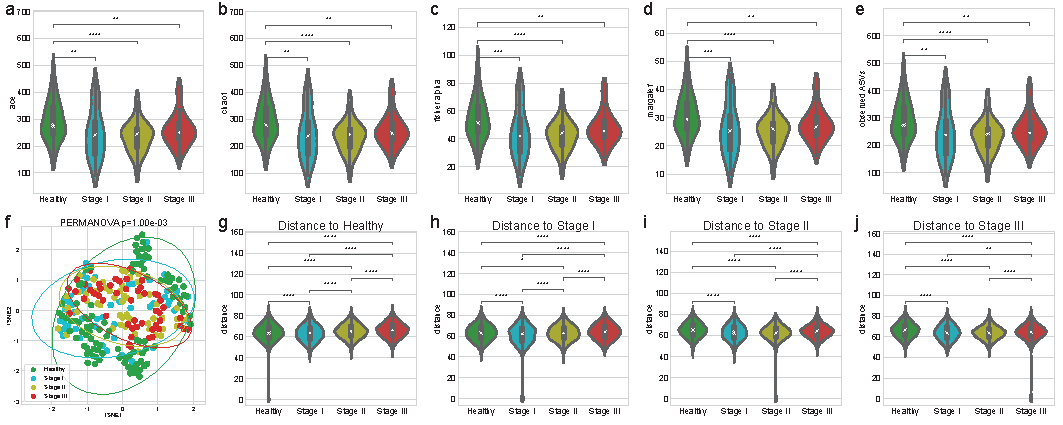
\includegraphics[width=\linewidth]{Figures/Periodontitis/Figure_1.pdf}
                \caption[Diversity indices]{\textbf{Diversity indices}. \\
                    Alpha-diversity indices \textbf{(a-e)} indicate that healthy controls have increased heterogeneity than periodontitis stages as measured by: \textbf{(a)} ACE \textbf{(b)} Chao1 \textbf{(c)} Fisher alpha \textbf{(d)} Margalef, and \textbf{(e)} observed ASVs. \textbf{(f)} The beta-diversity index (weighted UniFrac) was visualized using a tSNE-transformed plot. The confidence ellipses are shown to display the distribution of each periodontitis stage. The distance to each stage demonstrated that each periodontitis stage was distinguished from the other periodontitis stages: \textbf{(g)} distance to Healthy \textbf{(h)} distance to Stage I \textbf{(i)} distance to Stage II, and \textbf{(j)} distance to Stage III. Statistical significance determined by the MWU test and the PERMANOVA test: $p < 0.05$ (*), $p < 0.01$ (**), $p < 0.001$ (***), and $p \le 0.0001$ (****).}
                \label{fig:Periodontitis-diversity}
            \end{figure}
            \clearpage

            \begin{figure}[p]
                \centering
                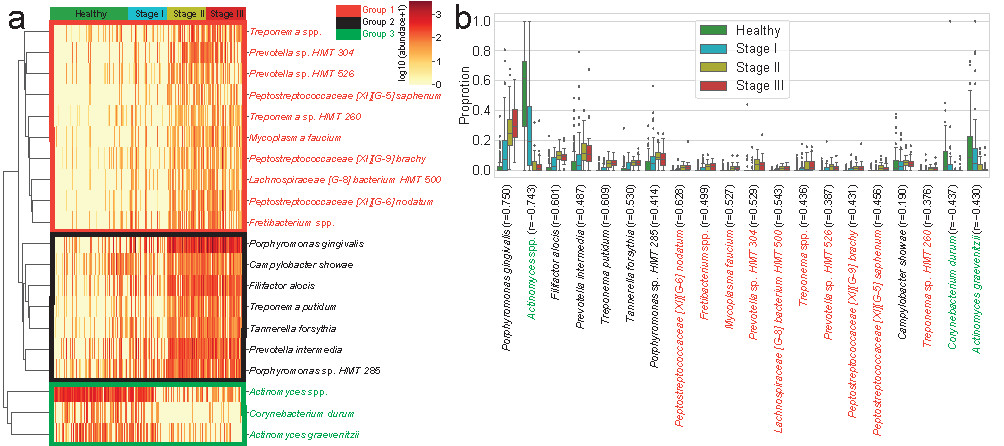
\includegraphics[width=\linewidth]{Figures/Periodontitis/Figure_2.pdf}
                \caption[Differentially abundant taxa (DAT)]{\textbf{Differentially abundant taxa (DAT)}. \\
                    DAT that were identified by ANCOM. \textbf{(a)} Heatmap of clustered DAT with similar distribution among subjects. Group 1, Group 2, and Group 3 are marked in red, black, and green, respectively. \textbf{(b)} Box plots showing the proportions of DAT. Taxa were sorted by their importance according to ANCOM.}
                \label{fig:Periodontitis-DAT}
            \end{figure}
            \clearpage

            \begin{figure}[p]
                \centering
                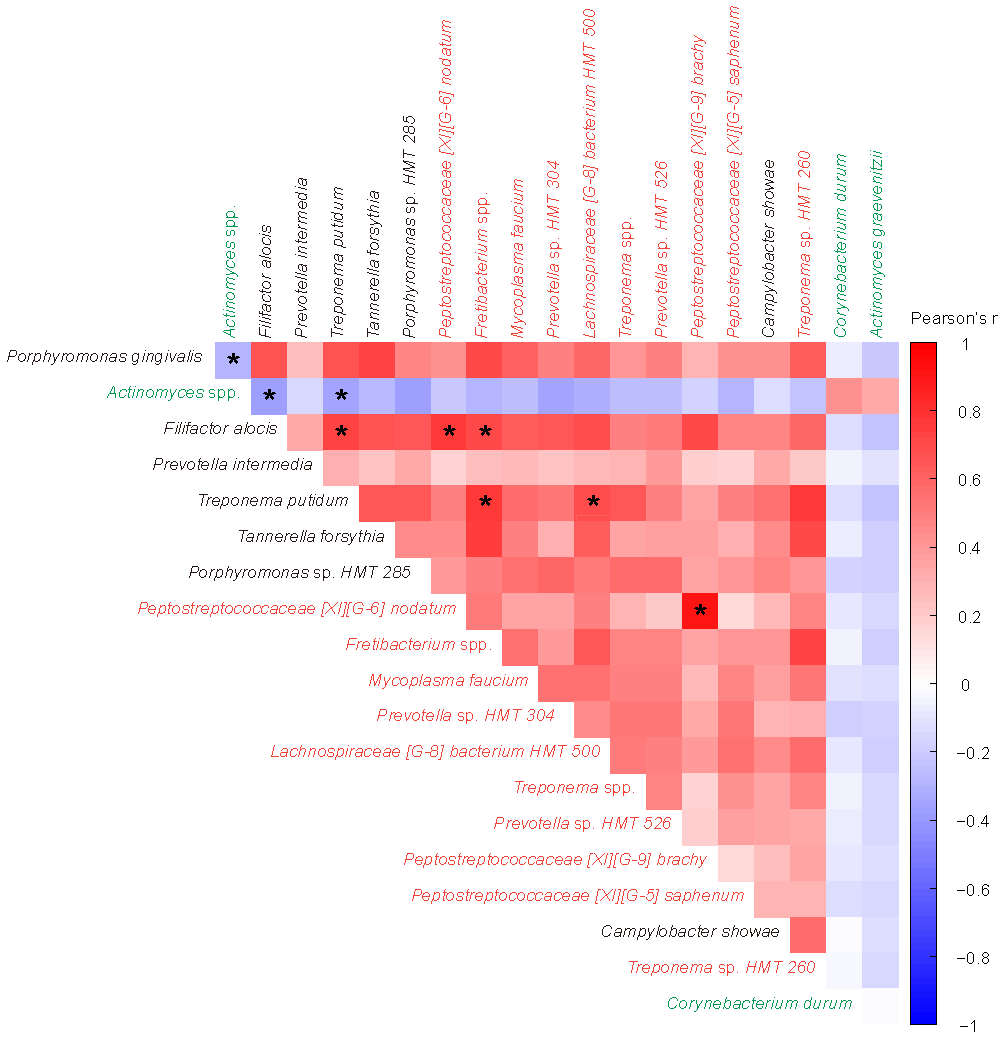
\includegraphics[width=\linewidth]{Figures/Periodontitis/Figure_3.pdf}
                \caption[Correlation heatmap]{\textbf{Correlation heatmap}. \\
                    Pearson's correlations between DAT in healthy status and periodontitis stages. Statistical significance was determined by strong correlation, i.e., $| \textrm{coefficient} | \ge 0.5$ (*).}
                \label{fig:Periodontitis-correlation}
            \end{figure}
            \clearpage

            \begin{figure}[p]
                \centering
                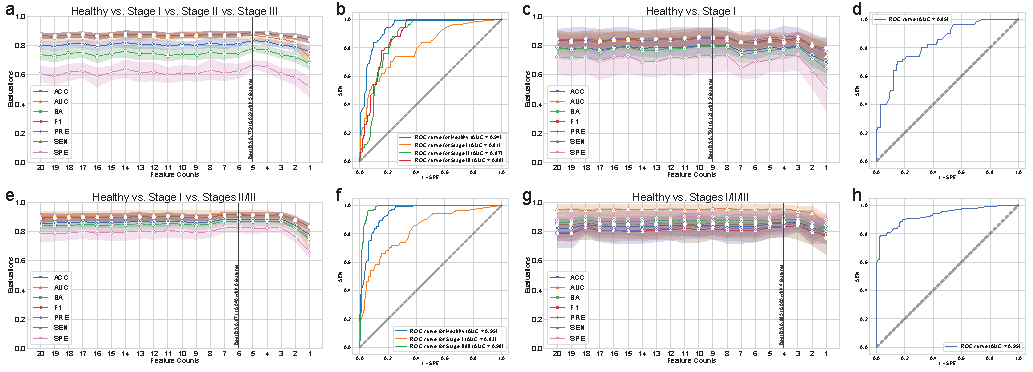
\includegraphics[width=\linewidth]{Figures/Periodontitis/Figure_4.pdf}
                \caption[Random forest classification metrics]{\textbf{Random forest classification metrics}. \\
                    The classification metrics in the random forest classifications were as follows: ACC, AUC, BA, F1, PRE, SEN, and SPE. \textbf{(a)} Classification performance for healthy vs. stage I vs. stage II vs. stage III. \textbf{(b)} ROC curve for the highest BA of (a). \textbf{(c)} Classification performance for healthy vs. stage I. \textbf{(d)} ROC curve on the highest BA of (c). (\textbf{e)} Classification performance for healthy vs. stage I vs. stages II/III. \textbf{(f)} ROC curve for the highest BA of (e). \textbf{(g)} Classification performance for healthy vs. stages I/II/III. \textbf{(h)} ROC curve for the highest BA of (h).}
                \label{fig:Periodontitis-ML}
            \end{figure}
            \clearpage

            \begin{figure}[p]
                \centering
                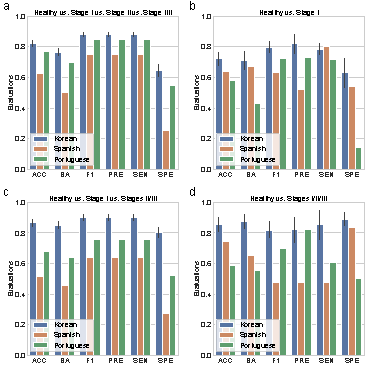
\includegraphics[width=\linewidth]{Figures/Periodontitis/Figure_5.pdf}
                \caption[Random forest classification metrics from external datasets]{\textbf{Random forest classification metrics from external datasets}. \\
                    The classification metrics in the random forest classifications were as follows: ACC, AUC, BA, F1, PRE, SEN, and SPE. \textbf{(a)} Classification performance for healthy vs. stage I vs. stage II vs. stage III. \textbf{(b)} Classification performance for healthy vs. stage I. \textbf{(c)} Classification performance for healthy vs. stage I vs. stages II/III. \textbf{(d)} Classification performance for healthy vs. stages I/II/III.}
                \label{fig:Periodontitis-validation}
            \end{figure}
            \clearpage

            \begin{figure}[p]
                \centering
                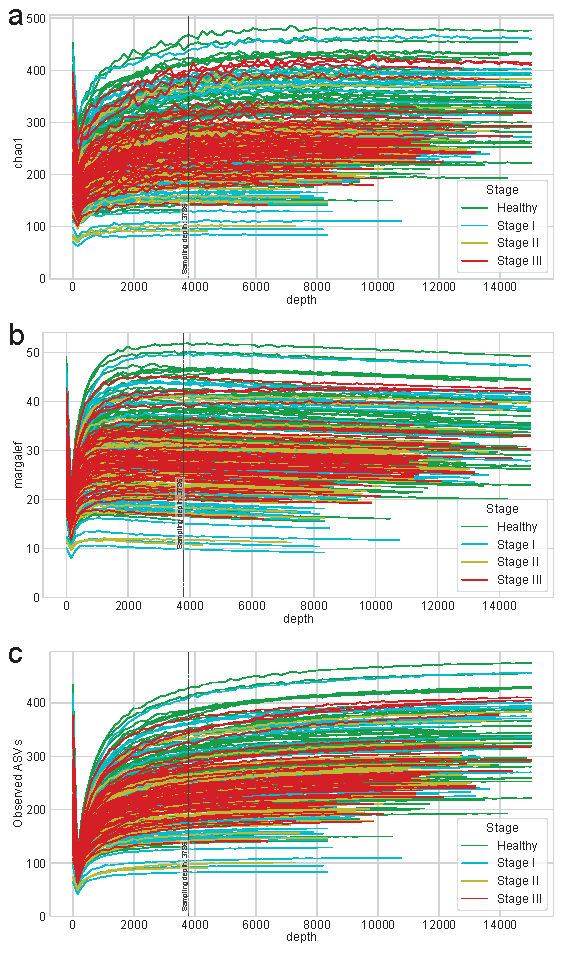
\includegraphics[width=0.75 \linewidth]{Figures/Periodontitis/Figure_S1.pdf}
                \caption[Rarefaction curves for alpha-diversity indices]{\textbf{Rarefaction curves for alpha-diversity indices}. \\
                    Rarefaction of \textbf{(a)} chao1 \textbf{(b)} margalef, and \textbf{(c)} observed ASVs were generated to measure species richness and determine the sampling depth of each sample.}
                \label{fig:Periodontitis-rarefaction}
            \end{figure}
            \clearpage

            \begin{figure}[p]
                \centering
                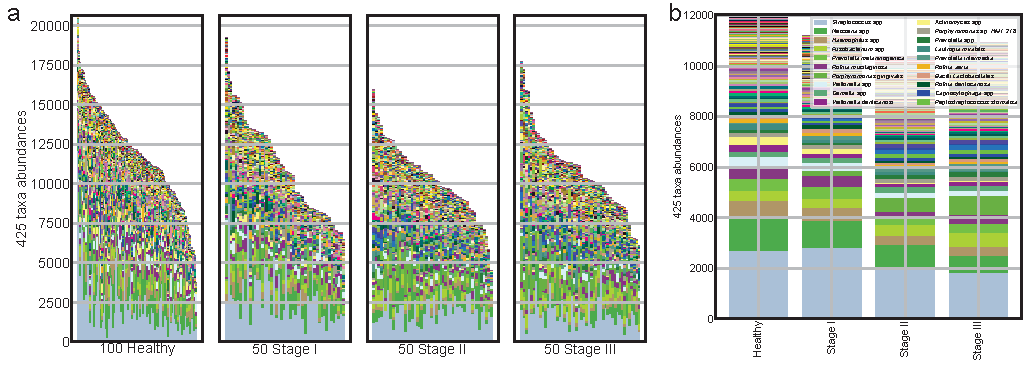
\includegraphics[width=\linewidth]{Figures/Periodontitis/Figure_S2.pdf}
                \caption[Salivary microbiome compositions in the different periodontal statuses]{\textbf{Salivary microbiome compositions in the different periodontal statuses}. \\
                    Stacked bar plot of the absolute abundance of bacterial species for all samples \textbf{(a)} and the mean absolute abundance of bacterial species in the healthy, stage I, stage II, and stage III groups \textbf{(b)}.}
                \label{fig:Periodontitis-abundance}
            \end{figure}
            \clearpage

            \begin{figure}[p]
                \centering
                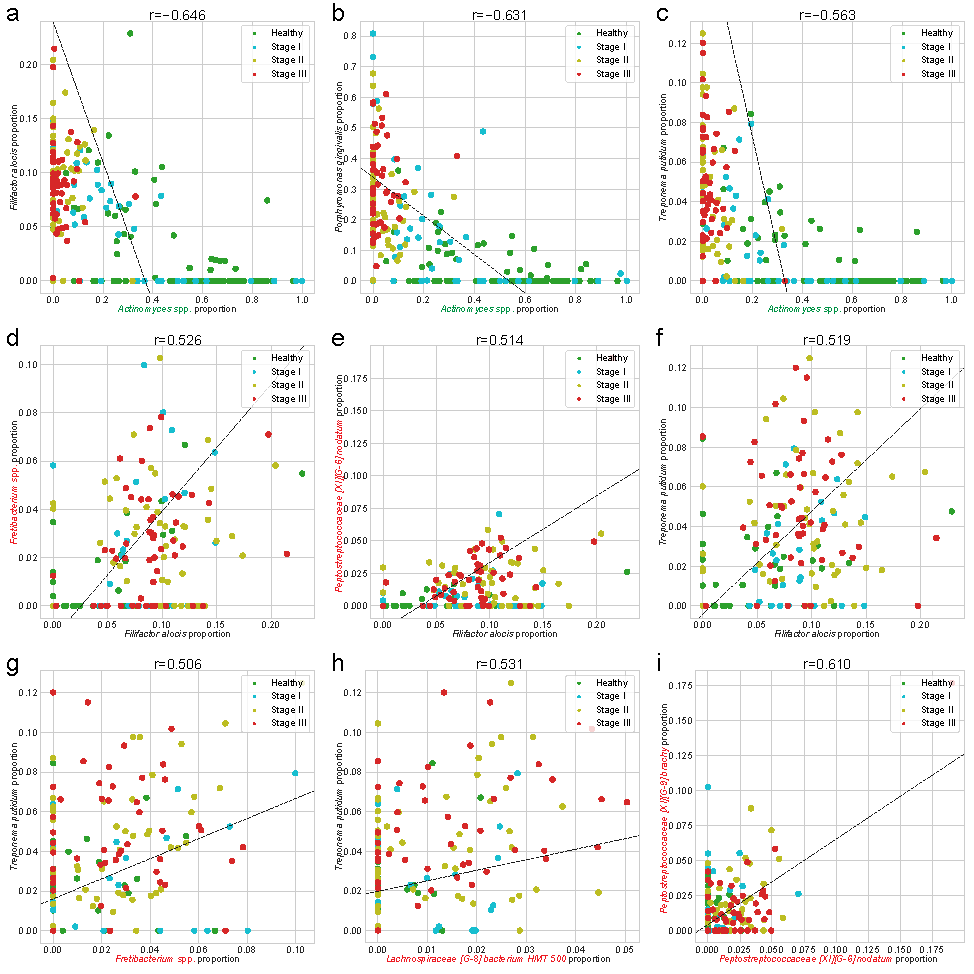
\includegraphics[width=\linewidth]{Figures/Periodontitis/Figure_S3.pdf}
                \caption[Correlation plots for differentially abundant taxa]{\textbf{Correlation plots for differentially abundant taxa}. \\
                    We selected the combinations of DAT with absolute Spearman correlation coefficients greater than 0.5. The color represents periodontal healthy periodontal statuses (green: healthy, cyan: stage I, yellow: stage II, and red: stage III).}
                \label{fig:Periodontitis-correlation2}
            \end{figure}
            \clearpage

            \begin{figure}[p]
                \centering
                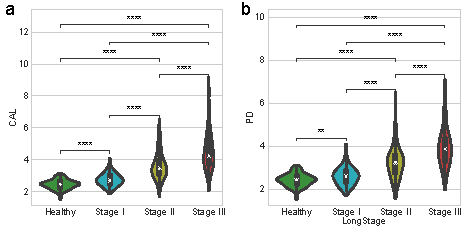
\includegraphics[width=\linewidth]{Figures/Periodontitis/Figure_R02.pdf}
                \caption[Clinical measurements by the periodontitis statuses]{\textbf{Clinical measurements by the periodontitis statuses}. \\
                    Comparisons of clinical measurement among healthy controls and patients with various periodontitis stages. \textbf{(a)} Clinical attachment level (CAL) \textbf{(b)} Probing depth (PD). Statistical significance determined by the MWU test: $p < 0.01$ (**) and $p < 0.0001$ (****).}
                \label{fig:Periodontitis-clinical}
            \end{figure}
            \clearpage

            \begin{figure}[p]
                \centering
                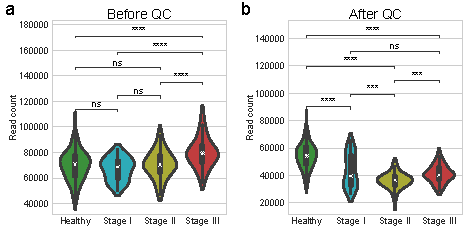
\includegraphics[width=\linewidth]{Figures/Periodontitis/Figure_R03.pdf}
                \caption[Number of read counts by the periodontitis statuses]{\textbf{Number of read counts by the periodontitis statuses}. \\
                    Comparisons of the number of read counts among healthy controls and patients with various periodontitis stages. \textbf{(a)} Before quality check \textbf{(b)} After quality check. Statistical significance determined by the MWU test: $p \ge 0.05$ (ns), $p < 0.05$ (*), $p < 0.01$ (**), $p < 0.001$ (***), and $p < 0.0001$ (****).}
                \label{fig:Periodontitis-QC}
            \end{figure}
            \clearpage

            \begin{figure}[p]
                \centering
                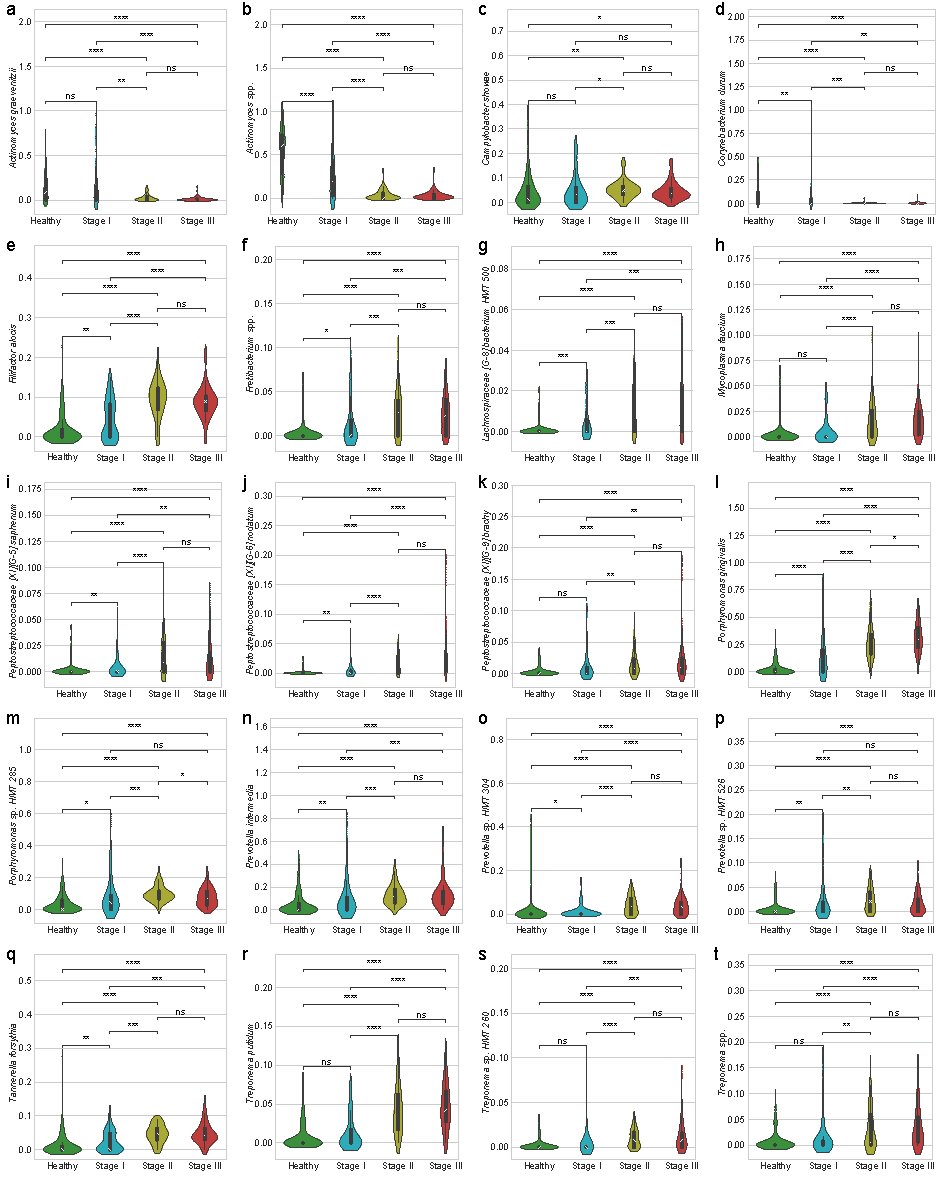
\includegraphics[width=0.9 \linewidth]{Figures/Periodontitis/Figure_R04.pdf}
                \caption[Proportion of DAT]{\textbf{Proportion of DAT}. \\
                    \textbf{(a)} \textit{Actinomyces graevenitzii} \textbf{(b)} \textit{Actinomyces} spp. \textbf{(c)} \textit{Campylobacter showae} \textbf{(d)} \textit{Corynebacterium durum} \textbf{(e)} \textit{Filifactor alocis} \textbf{(f)} \textit{Fretibacterium} spp. \textbf{(g)} \textit{Lachnospiraceae [G-8] bacterium HMT 500} \textbf{(h)} \textit{Mycoplasma faucium} \textbf{(i)} \textit{Peptostreptococcaceae [XI][G-5] saphenum} \textbf{(j)} \textit{Peptostreptococcaceae [XI][G-6] nodatum} \textbf{(k)} \textit{Peptostreptococcaceae [XI][G-9] brachy} \textbf{(l)} \textit{Porphyromonas gingivalis} \textbf{(m)} \textit{Porphyromonas} sp. \textit{HMT 285} \textbf{(n)} \textit{Prevotella intermedia} \textbf{(o)} \textit{Prevotella} sp. \textit{HMT 304} \textbf{(p)} \textit{Prevotella} sp. \textit{HMT 526} \textbf{(q)} \textit{Tannerella forsythia} \textbf{(r)} \textit{Treponema putidum} \textbf{(s)} \textit{Treponema} sp. \textit{HMT 260} \textbf{(t)} \textit{Treponema} spp. Statistical significance determined by the MWU test: $p \ge 0.05$ (ns), $p < 0.05$ (*), $p < 0.01$ (**), $p < 0.001$ (***), and $p < 0.0001$ (****).}
                \label{fig:Periodontitis-proportions}
            \end{figure}
            \clearpage

            \begin{figure}[p]
                \centering
                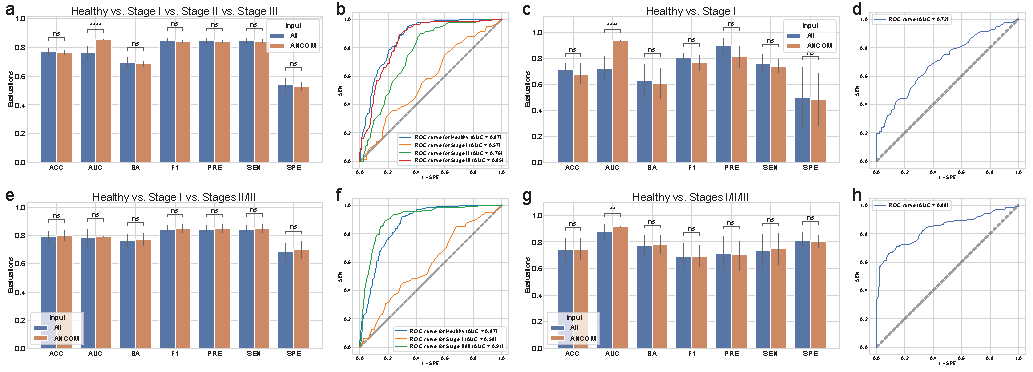
\includegraphics[width=\linewidth]{Figures/Periodontitis/Figure_R05.pdf}
                \caption[Random forest classification metrics with the full microbiome compositions and ANCOM-selected DAT compositions]{\textbf{Random forest classification metrics with the full microbiome compositions and ANCOM-selected DAT compositions}. \\
                    The classification metrics in the random forest classifications were as follows: ACC, AUC, BA, F1, PRE, SEN, and SPE. \textbf{(a)} Classification performance for healthy vs. stage I vs. stage II vs. stage III. \textbf{(b)} ROC curve for the highest BA of (a). \textbf{(c)} Classification performance for healthy vs. stage I. \textbf{(d)} ROC curve on the highest BA of (c). \textbf{(e)} Classification performance for healthy vs. stage I vs. stages II/III. \textbf{(f)} ROC curve for the highest BA of (e). \textbf{(g)} Classification performance for healthy vs. stages I/II/III. \textbf{(h)} ROC curve for the highest BA of (g). Statistical significance determined by the MWU test: $p \ge 0.05$ (ns), $p < 0.01$ (**), and $p < 0.0001$ (****).}
                \label{fig:Periodontitis-full}
            \end{figure}
            \clearpage

            \begin{figure}[p]
                \centering
                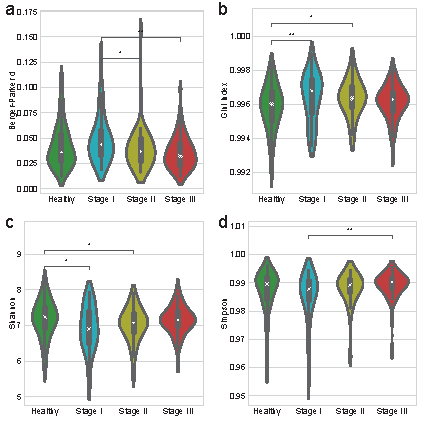
\includegraphics[width=\linewidth]{Figures/Periodontitis/Figure_R06.pdf}
                \caption[Alpha-diversity indices account for evenness]{\textbf{Alpha-diversity indices account for evenness}. \\
                    Alpha-diversity indices \textbf{(a-d)} indicate that the heterogeneity between the periodontitis stages as measured by: \textbf{(a)} Berger-Parker $d$ \textbf{(b)} Gini \textbf{(c)} Shannon \textbf{(d)} Simpson. Statistical significance determined by the MWU test: $p < 0.05$ (*) and $p < 0.01$ (**)}
                \label{fig:Periodontitis-alpha}
            \end{figure}
            \clearpage

            \begin{figure}[p]
                \centering
                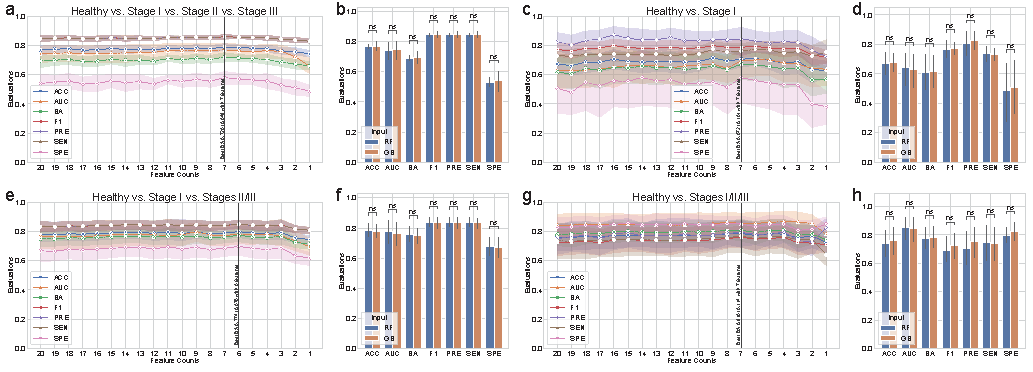
\includegraphics[width=\linewidth]{Figures/Periodontitis/Figure_R09.pdf}
                \caption[Gradient Boosting classification metrics]{\textbf{Gradient Boosting classification metrics}. \\
                    The classification metrics in the random forest classifications were as follows: ACC, AUC, BA, F1, PRE, SEN, and SPE. The feature counts mean that the classification model trained on the most important $n$ features as the Table \ref{tab:Periodontitis-DAT}. \textbf{(a)} Comparison of Random forest (RF) and Gradient boosting (GB) for healthy vs. stage I vs. stage II vs. stage III. \textbf{(b)} Comparison of RF and GB for the highest BA of (a). \textbf{(c)} Classification performance for healthy vs. stage I. \textbf{(d)} Comparison of RF and GB for healthy vs. stage I vs. stages II/III. \textbf{(e)} Comparison of RF and GB for the highest BA of (d). \textbf{(f)} Comparison of RF and GB for Healthy vs. Stage I vs. Stages II/III. \textbf{(g)} Classification performance for healthy vs. stages I/II/III. \textbf{(h)} Comparison of RF and GB for Healthy vs. Stages I/II/III. MWU test: $p \ge 0.05$ (ns)}
                \label{fig:Periodontitis-GB}
            \end{figure}
            \clearpage
        \newpage

        \subsection{Discussion}
            In order to investigate at potential alterations in the salivary microbiome compositions based on periodontal statuses, including healthy, stage I, stage II, and stage III, we employed 16S rRNA gene sequencing to perform a cross-sectional periodontitis analysis. In this study, the 2018 periodontitis classification served as the basis for the classification of periodontitis severities \cite{Periodontitis-4}. There were notable variations in the salivary microbiome composition among the multiple severities of periodontitis (Figure \ref{fig:Periodontitis-abundance}). Furthermore, our random forest classification model based on the proportions of DAT in the salivary microbiome compositions across study participants to predict multiple periodontitis statuses with high AUC of 0.870$\pm$0.079 (Table \ref{tab:Periodontitis-ML}).

            Previous research identified the red complex as the primary pathogens of periodontitis \cite{Periodontitis-14}: \textit{Porphyromonas gingivalis}, \textit{Tannerella forsythia}, and \textit{Treponema denticola}. Other studies, however, have shown that periodontal pathogens communicate with other bacteria in the salivary microbiome networks to generate dental plaque prior to the pathogenesis and development of periodontitis \cite{Periodontitis-15, Periodontitis-16, Periodontitis-17}.

            Using subgingival plaque collections, recent researches have suggested a connection between the periodontitis severity and the salivary microbiome compositions \cite{Periodontitis-9, Periodontitis-10, Periodontitis-11}. Therefore, we have examined the salivary microbiome compositions of patients with multiple severities of periodontitis and periodontally healthy controls, extending on earlier studies.

            According to our findings, the salivary microbiome compositions have 425 taxa (Figure \ref{fig:Periodontitis-abundance}). We computed the alpha-diversity indices to determine the variability within each salivary microbiome composition, including ace \cite{ACE-1}, chao1 \cite{chao1-1}, fisher alpha \cite{fisher-1}, margalef \cite{margalef-1}, observed ASVs \cite{observed-ASVs-1}, Berger-Parker $d$ \cite{Berger-1}, Gini index \cite{Gini-1}, Shannon \cite{Shannon-1}, and Simpson \cite{Simpson-1} (Figure \ref{fig:Periodontitis-diversity} and Figure \ref{fig:Periodontitis-alpha}). Alpha-diversity indices suggested that the microbial richness of periodontally healthy controls was higher than that of patients with periodontitis (Figure \ref{fig:Periodontitis-diversity}a-e and Figure \ref{fig:Periodontitis-alpha}). These results are in line with findings with that patients with advanced periodontitis, namely stage II and stage III, have less diversified communities than periodontally healthy controls \cite{Periodontitis-18}. Recognizing that the periodontitis severity increases the amount of \textit{Porphyromonas gingivalis}, the salivary microbiome compositions from periodontally healthy controls conserved microbial networks dominated by \textit{Streptococcus} spp. (Figure \ref{fig:Periodontitis-abundance}). \textit{Porphyromonas gingivalis} is one of the known periodontal pathogen that could cause dysbiosys in the salivary microbiomes, suggesting in the pathophysiology of periodontitis. Despite this finding, earlier research found that subgingival microbiome of patients with periodontitis had a greater alpha-diversity index (observed ASVs) than that of healthy controls \cite{Periodontitis-10}, might due to the different sampling sites between saliva and subgingival plaque. On the other hand, another research has addressed significant discrepancies in alpha-diversity indices from subgingival plaque, saliva, and tongue biofilms from healthy controls and periodontitis patients, resulting the highest alpha-diversity index in saliva collections \cite{Periodontitis-19}. Moreover, early-stage periodontitis, namely stage I, did not determine statisticall ysignificant differences in alpha-diversity indices compared to advanced periodontitis, including stage II and stage III (Figure \ref{fig:Periodontitis-diversity}a-e). Accordingly, saliva collection of stage I periodontitis may exhibit heterogeneity, indicating a midpoint condition between a healthy state and advanced periodontitis (stage II and stage III). Likewise, gingivitis is often associated with low abundances of the majority of periodontal pathogens, including \textit{Porphyromonas gingivalis}, \textit{Tannerella forsythia}, and \textit{Treponema denticola} \cite{Periodontitis-7}. Compared to healthy controls, patients with stage I periodontitis have higher detection rates of \textit{Porphyromonas gingivalis} and \textit{Tannerella forsythia} \cite{Periodontitis-20, Periodontitis-21}.

            Therefore, we calculated beta-diversity indices to analyze the differences between the study participants. The distances for the multiple stages of periodontitis, including stage I, stage II, and stage III, as well as healthy controls (Figure \ref{fig:PTB-diversity}g-j and Table \ref{tab:Periodontitis-beta}), suggesting notable differences among the multiple periodontitis severities. In other words, the composition of the salivary microbiome compositions varies depending on the periodontitis stages, so that supporting the findings from a previous study \cite{Periodontitis-10}. Taken together that it is nearly impossible to fully restore the attachment level after it has been lost due to the progression and development of periodontitits, the ability to rapidly screen for periodontitis in its early phases using saliva collections would be highly beneficial for effective disease management and treatment.

            Of the total of 425 taxa in the salivary microbiome composition that have been identified (Figure \ref{fig:Periodontitis-abundance}), ANCOM was applied to select 20 taxa as the DAT that indicated notable abundance variation among the periodontitis severities (Figure \ref{fig:Periodontitis-DAT} and Table \ref{tab:Periodontitis-DAT}). Three sub-groups were formed from the DAT using hierarchical clustering (Figure \ref{fig:Periodontitis-DAT}a). Surprisingly, two of the red complex pathogens \cite{Periodontitis-22}, \textit{Porphyromonas gingivalis} and \textit{Tannerella forsythia}, were classified in Group 2 and were more prevalent in stage II and stage II periodontitis compared to healthy controls. \textit{Campylobacter showae} was additionally placed in Group 2 of the orange complex pathogens \cite{Periodontitis-23}. Furthermoe, some of the DAT in Group 2 have reported their crucial roles in pathogenesis and development of periodontitis: \textit{Filifactor alocis} \cite{Periodontitis-24}, \textit{Treponema putidum} \cite{Periodontitis-25}, \textit{Tannerella forsythia} \cite{Periodontitis-26, Periodontitis-27}, and \textit{Prevotella intermedia} \cite{Periodontitis-28}. Taken together, this indicates that DAT in Group 2 is essential to periodontitis. The portion of some Group 1 DAT, including \textit{Peptostreptococcaceae[XI][G-5] saphenum}, \textit{Peptostreptococcaceae[XI][G-6] nodatum}, and \textit{Peptostreptococcaceae[XI][G-9] brachy}, in healthy controls and patients with periodontitis significantly differed, according to earlier research \cite{Periodontitis-8}. These outcomes support our research, implying that Group 1 DAT are also essential to the etiology and progression of periodontitis. However, in contrast to patients with periodontitis, Group 3 DAT, namely \textit{Corynebacterium durum} and \textit{Actinomyces graevenitzii},  were enriched in healthy controls, which is consistent with earlier research \cite{Periodontitis-29, Periodontitis-30}.

            In our correlation analysis (Figure \ref{fig:Periodontitis-correlation}), we have discovered strongly negative correlations ($\textrm{coefficient} \le -0.5$) between DAT of Group 3 and these of Group 1 and Group 2; we have also identified nine DAT pairs with strong correlations ($\textrm{coefficient} \le -0.5 \vee \textrm{coefficient} \ge 0.5$) (Figure \ref{fig:Periodontitis-correlation2}). Interestingly, there were strongly negative correlations ($\textrm{coefficient} \le -0.5$) between Group 2 DAT and \textit{Actinomyces} spp., taxa which belong to Group 3: \textit{Filifactor alocis} (Figure \ref{fig:Periodontitis-correlation2}a), \textit{Porphyromonas gingivalis} (Figure \ref{fig:Periodontitis-correlation2}b), and \textit{Treponema putidum} (Figure \ref{fig:Periodontitis-correlation2}c). Taken together that pathogens, including \textit{Filifactor alocis} \cite{Periodontitis-31, Periodontitis-32}, \textit{Porphyromonas gingivalis} \cite{Periodontitis-22}, and \textit{Treponema putidum} \cite{Periodontitis-25}, become dominant taxa in patients with stage III periodontitis. On the other hand, commensal salivary bacteria, such as \textit{Actinomyces} spp., gradually declined. Additionally, several DAT from Group 1 and Group 2 exhibited strong positive correlations ($\textrm{coefficient} \ge 0.5$) (Figure \ref{fig:Periodontitis-correlation2}d-i). It has been established that all of these DAT from Group 1 and Group 2 are periodontal pathogens: \textit{Filifactor alocis} \cite{Periodontitis-31, Periodontitis-32}, \textit{Fretibacterium} spp. \cite{Periodontitis-33}, \textit{Lachnospiraceae[G-8] bacterium HMT 500} \cite{Periodontitis-8}, \textit{Peptostreptococcaceae[XI][G-6] nodatum} \cite{Periodontitis-8, Periodontitis-34}, \textit{Peptostreptococcaceae[XI][G-9] brachy} \cite{Periodontitis-8}, and Treponema putidum \cite{Periodontitis-25}. Thus, these fundamental roles of identified periodontal pathogens in the pathophysiology and progression of periodontitis are further supported by these strong positive correlations ($\textrm{coefficient} \ge 0.5$), suggesting that advanced periodontitis, \textit{i.e.}, stage III, might arise from the additional DAT from Group 1 and Group 2.

            Moreover, to predict peridontitis statuses from salivary microbiome composition, we have constructed machine-learning classification models based on random forest for four classification settings:
            \begin{enumerate}[noitemsep,nolistsep]
                \item healthy vs. stage I vs. stage II vs. stage III
                \item healthy vs. stage I
                \item healthy vs. stage I vs. stages II/III
                \item healthy vs. stages I/II/III
            \end{enumerate}
            \textit{Porphyromonas gingivalis} and \textit{Actinomyces} spp. were the two most important taxa (feature) in all classification settings. This finding aligns with a recent study that identifies \textit{Actinomyces} spp. as the most prevalent bacteria in both the healthy gingivitis controls, while \textit{Porphyromonas gingivalis} is recognized as the most predominant taxon within the periodontitis subjects, based on analyses of subgingival plaque samples \cite{Periodontitis-11}. We have previously developed machine learning models for the classification of periodontitis, with the objective of predicting the severities of chronic periodontitis by analyzing the copy numbers of nine known salivary bacteria species. We classified healthy controls and patients with periodontitis utilizing bacterial combinations in conjunction with a random forest model \cite{Periodontitis-diagnosis-8}:
            \begin{itemize}[noitemsep,nolistsep]
                \item AUC: 94\%
                \item BA: 84\%
                \item SEN: 95\%
                \item SPE: 72\%
            \end{itemize}

            Another study established a machine-learning model for the classification of periodontitis, employing 266 species derived from the buccal microbiome \cite{Periodontitis-35}:
            \begin{itemize}[noitemsep,nolistsep]
                \item AUC: 92\%
                \item BA: 84\%
                \item SEN: 94\%
                \item SPE: 74\%
            \end{itemize}

            By separating patients with periodontitis from healthy controls using only four DAT, \textit{e.g.} \textit{Actinomyces graevenitzii}, \textit{Actinomyces} spp., \textit{Corynebacterium durum}, and \textit{Porphyromonas gingivalis}, our machine learning model performed better than previously published models (Figure \ref{fig:Periodontitis-ML}, Table \ref{tab:Periodontitis-ML}, and Table \ref{tab:Periodontitis-importance}):
            \begin{itemize}[noitemsep,nolistsep]
                \item AUC: 95.3\%$\pm$4.9\%
                \item BA: 88.5\%$\pm$6.6\%
                \item SEN: 86.4\%$\pm$15.7\%
                \item SPE: 90.5\%$\pm$7.0\%
            \end{itemize}

            This result showed that by detecting Group 3 bacteria that were substantially abundant in health controls than patients with periodontitis, our study increased BA by at least 5\% and SPE by at least 17\%.

            Furthermore, we have validated our machine-learning prediction model using openly accessible 16S gene rRNA sequencing data from Portuguese \cite{Periodontitis-10} and Spanish participants \cite{Periodontitis-Portuguese-1} in order to ensure the consistency of our random forest classification model (Figure \ref{fig:Periodontitis-validation}). Our classification models employed in this study were primarily developed and assessed on Korean study participants, which may limit their generalizability to other ethnic groups with different salivary microbiome compositions \cite{Periodontitis-ethnic-1, Periodontitis-ethnic-2}. Therefore, the evaluations of this periodontitis classification models can be affected by ethnic-specific variances and differences, highlighting the necessity for additional validation and adjustment across a spectrum of ethnic backgrounds.

            Regarding the clinical characteristics and potential confounders influencing the analysis of salivary microbiome compositions connected with periodontitis severity, this study had a number of limitations that were pointed out. We did not offer clinical information, such as the percentage of teeth, the percentage of bleeding on probing, nor dental furcation involvement, even though we did gather information on attachment level, probing depth, plaque index, and gingival index \cite{Periodontitis-diagnosis-9}; this might have it challenging to present thorough and in-depth data about periodontal health. Moreover, the broad age range may make it tougher to evaluate the relationship between age and periodontitis statuses, providing the necessity for future studies to consider into account more comprehensive clinical characteristics associated with periodontitis. Additionally, potential confounders--\textit{e.g.} body mass index \cite{obesity-1} and e-cigarette use \cite{cigarette-1}--which might have affected dental health and salivary microbiome composition were disregarding consideration in addition to smoking status and systemic diseases. Thus, future research incorporating these components would offer a more thorough knowledge of how lifestyle factors interact and affect the salivary microbiome composition and periodontal health. Throughout, resolving these limitations will advance our understanding in pathogenesis and development of periodontitis, offering significant novel insights on the causal connection between systemic diseases and the salivary microbiome compositions.
        \newpage

    \section{Metagenomic signature analysis of Korean colorectal cancer}
        \label{section:CRC}
        \subsection{Introduction}
            Colorectal cancer (CRC) is one of the most prevalent and life-threatening malignancies worldwide \cite{CRC-1, CRC-2, CRC-3}, with its incidence influenced by a combination of genetic \cite{CRC-factor-1, CRC-factor-2}, environmental \cite{CRC-factor-3, CRC-factor-4}, and lifestyle factors \cite{CRC-factor-5, CRC-factor-6, CRC-factor-7, CRC-factor-8}. Established risk factors include a often diet in red and processed meats \cite{CRC-factor-9, CRC-factor-10}, obesity \cite{CRC-factor-11, CRC-factor-12}, cigarette smoking \cite{CRC-factor-5, CRC-factor-6}, alcohol consumption \cite{CRC-factor-7, CRC-factor-8}, and a sedentary lifestyle \cite{CRC-factor-13}, all of which contribute to chronic inflammation, mutagenesis, and metabolic regulation. Additionally, underlying conditions, \textit{e.g.} Lynch syndrome \cite{CRC-disease-3, CRC-disease-4} and familial adenomatous polyposis \cite{CRC-disease-1, CRC-disease-2}, significantly increase risk of CRC due to persistent mucosal inflammation and somatic mutations that promote tumorigenesis.

            The gut microbiome plays a fundamental role in maintaining host health by helping digestion \cite{gut-digestion-1, gut-digestion-2}, regulating metabolism \cite{gut-metabolism-1, gut-metabolism-2, gut-metabolism-3}, adjusting immune function \cite{gut-immune-1, gut-immune-2, gut-immune-3}, and even coordinating neurological processes by the brain-gut axis \cite{brain-gut-1, brain-gut-2, brain-gut-3}. Comprising these gut microbiota, including, archaea, bacteria, fungi, and viruses, the gut microbiome contributes to the synthesis of essential vitamins, and production of fatty acids, which influence intestinal integrity and immune responses. Thus, well-balanced gut microbiome composition modulates systemic immune function by interacting with gut-associated lymphoid tissue, shaping immune tolorence and response to infections. Hence, emerging evidence suggests that dysbiosis in the gut microbiome composition are associated not only a narrow range of diseases, \textit{e.g.} diarrhea and enteritis \cite{gut-diarrhea-1, gut-diarrhea-2} but also a wide range of diseases, \textit{e.g.} obesity, diabetes, and cancers \cite{microbiome-diabetes-1, microbiome-diabetes-2, microbiome-cancer-1, microbiome-cancer-2}.

            Recent studies have highlighted the crucial role of the gut microbiome in tumorigenesis and progression of CRC \cite{gut-CRC-1, gut-CRC-2}, with dysbiosis emerging as a potential risk factor. Dysbiosis in gut microbiome compositions can promote tumorigenesis of many cancers, including CRC, through several signaling cascades, including inflammation, mutagenesis, and altered metabolism in host. Certain bacteria species, such as \textit{Fusobacterium} genus \cite{Fusobacterium-5, Fusobacterium-6, Fusobacterium-7}, \textit{Bacteroides} genus \cite{Bacteroides-1, Bacteroides-2}, and \textit{Escherichia coli} \cite{Escherichia-1, Escherichia-2}, have been associated with development and progression of CRC by producing pro-inflammatory signals, generating toxins including mutagens, and disrupting the intestinal barriers including mucous surface. In contrast, beneficial bacteria, such as \textit{Lactobacillus} genus \cite{Lactobacillus-1, Lactobacillus-2} and \textit{Bifidobacterium} genus \cite{Bifidobacterium-1, Bifidobacterium-2}, are regarded to apply protective roles by maintaining homeostasis of gut microbiome compositions and regulating immune responses including inflammation.

            Furthermore, identifying metagenome biomarkers in Korean CRC patients is essential, as the gut microbiome compositions significantly vary by ethnicity due to genetic, dietary, and environmental factor \cite{CRC-ethnic-1, CRC-ethnic-2, CRC-ethnic-3}. Additionally, ethnicity-specific microbiome composition signatures may affect the reliability of previously established biomarkers derived from predominantly Western CRC cohorts \cite{CRC-TCGA-1}, necessitating population-specific investigations. By identifying metagenomic biomarkers tailored to Korean CRC patients, we can improve early detection rate of early-stage CRC, develop more accurate risk of CRC, and explore microbiome-targeted therapies that consider host-microbiome interactions within the Korean population.

            Accordingly, this study aims to identify microbiome-based biomarkers specific to CRC within the Korean population, addressing the critical demand for ethnicity-specific microbiome research. By leveraging metagenomic sequencing and advanced computational biology analysis, this study seeks to uncover novel microbial signatures associated with Korean CRC patients. As part of the larger "Multi-genomic analysis for biomarker development in colon cancer" project (NTIS No. \texttt{1711055951}), this study investigates microbial signatures within next-generation sequencing data to enhance precision medicine approaches for CRC and to develop robust microbiome-based biomarkers for early detection, prognosis, and therapeutic stratification, complementing genomic and epigenomic markers. Hence, this research represents a crucial step toward personalized cancer diagnostic and therapeutic strategies tailored to the Korean population.
        \clearpage

        \subsection{Materials and methods}
            \subsubsection{Study participants enrollment}
                To achieve metagenomic observations of CRC, a total of 211 Korean CRC patients were enrolled (Table \ref{tab:CRC-clinical}). The tissue samples were collected from both the tumor lesion and its corresponding adjacent normal lesion to enable comparative metagenomic analyses. Tumor tissue samples were obtained from confirmed CRC lesions, ensuring adequate representation of CRC-associated microbial alterations. Adjacent normal tissues were collected from non-cancerous regions away from the tumor margin to serve as a control for baseline molecular and microbial composition. Moreover, clinical information was collected for all study participants included in this study to investigate potential associations between gut microbiome compositions and clinical outcomes. Key clinical characteristics recorded included overall survival (OS), recurrence, age at diagnosis and sex. Additionally, microsatellite instability (MSI) status, a critical molecular feature of CRC \cite{CRC-MSI-1, CRC-MSI-2, CRC-MSI-3}, was evaluated using next-generation sequencing methods to classify CRC as MSI-high, MSI-low, or microsatellite stable (MSS). These clinical parameters were integrated with metagenomic data to explore potential microbiome-based biomarkers for CRC prognosis and progression. Ethical approval was obtained for clinical data collection, and all patient information was anonymized to ensure confidentially in accordance with institutional guidelines.

            \subsubsection{DNA extraction procedure}
                Tissue samples were immediately processed under sterile conditions to prevent contamination and preserved in low temperature ($-$80 \textcelsius) storage for downstream DNA extraction and whole-genome sequencing. Furthermore, produced sequencing data were provided by the "Multi-genomic analysis for biomarker development in colon cancer" project (NTIS No. \texttt{1711055951}) in mapped BAM format, aligned to the hg38 human reference genome. The preprocessing pipeline utilized by the main project included high-throughput whole-genome sequencing using standardized alignment algorithm, BWA \cite{BWA-1}. In addition to the mapped human sequences, our whole-genome sequencing data retained unmapped sequences, which contain potential microbial reads that were not aligned to the human reference genome.

            \subsubsection{Bioinformatics analysis}
                To identify microbial signatures associated with CRC, we employed PathSeq (version 4.1.8.1) \cite{PathSeq-1, PathSeq-2}, a computational pipeline designed for metagenomic analysis of high-throughput sequencing data including the whole-genome sequences. After processing these sequencing data through the PathSeq pipeline, a comprehensive bioinformatics analyses were conducted to characterize microbial signatures associated with CRC.

                Prevalent taxa identification was performed by determining microbial taxa present in the majority of the study participants, filtering out low-abundance and rare taxa to ensure robust downstream analyses.

                To assess microbial community structure, diversity indices were calculated, including alpha-diversity to evaluate single-sample diversity and beta-diversity to compare microbial composition between the tumor tissues and their corresponding adjacent normal tissues. Following alpha-diversity indices were calculated using the scikit-bio Python package (version 0.6.3) \cite{scikit-bio-1}, and these alpha-diversity indices were compared using the MWU test:
                \begin{enumerate}[noitemsep, nolistsep]
                    \item Berger-Parker $d$ \cite{Berger-1}
                    \item Chao1 \cite{chao1-1}
                    \item Dominance
                    \item Doubles
                    \item Fisher \cite{fisher-1}
                    \item Good’s coverage \cite{goods-1}
                    \item Margalef \cite{margalef-1}
                    \item Mcintosh $e$ \cite{mcintosh-1}
                    \item Observed ASVs \cite{observed-ASVs-1}
                    \item Simpson $d$
                    \item Singles
                    \item Strong \cite{strong-1}
                \end{enumerate}

                Furthermore, these beta-diversity indices were measured and compared using the PERMANOVA test \cite{PERMANOVA-1, PERMANOVA-2}. To demonstrate multi-dimensional data from the beta-diversity indices, we utilized the t-SNE algorithm \cite{tSNE-1}.
                \begin{enumerate}[noitemsep, nolistsep]
                    \item Bray-Curtis \cite{BrayCurtis-1}
                    \item Canberra
                    \item Cosine \cite{Cosine-1}
                    \item Hamming \cite{Hamming-1}
                    \item Jaccard \cite{Jaccard-1}
                    \item Sokal-Sneath \cite{Sokal-1}
                \end{enumerate}

                Differentially abundant taxa (DAT) were identified using statistical method, (DESeq2 \cite{DESeq2-1}, ANCOM \cite{ANCOM-1}), adjusting for sequencing depth and potential confounders to highlight taxa significantly associated with CRC. To explore functional implications, microbial pathway prediction was performed using (PICRUSt3, HUMAnN3), linking microbial composition to metabolic and functional pathways relevant to carcinogenesis and progression of CRC. This multi-layered bioinformatics approach enabled a comprehensive investigation of gut microbiome alteration in CRC, facilitating the identification of potential microbial biomarkers for diagnosis and prognosis of CRC.

            \subsubsection{Data and code availability}
                All sequences from the 211 study participants have been published to the Korea Bioinformation Center (data ID \texttt{KGD10008857}): \url{https://kbds.re.kr/KGD10008857}.
                Docker image that employed throughout this study is available in the DockerHub: \url{https://hub.docker.com/repository/docker/fumire/unist-crc-copm/general}. Every code used in this study can be found on GitHub: \url{https://github.com/CompbioLabUnist/CoPM-ColonCancer}.
        \clearpage

        \subsection{Results}
            \subsubsection{Summary of clinical characteristics}
            \subsubsection{Gut microbiome compositions}
            \subsubsection{Diversity indices}
            \subsubsection{DAT selection}
            \subsubsection{ML prediction}

            \begin{table}[p]
                \caption{Clinical characteristics of CRC study participants}
                \label{tab:CRC-clinical}
            \end{table}
            \clearpage

            \begin{figure}[p]
                \centering
                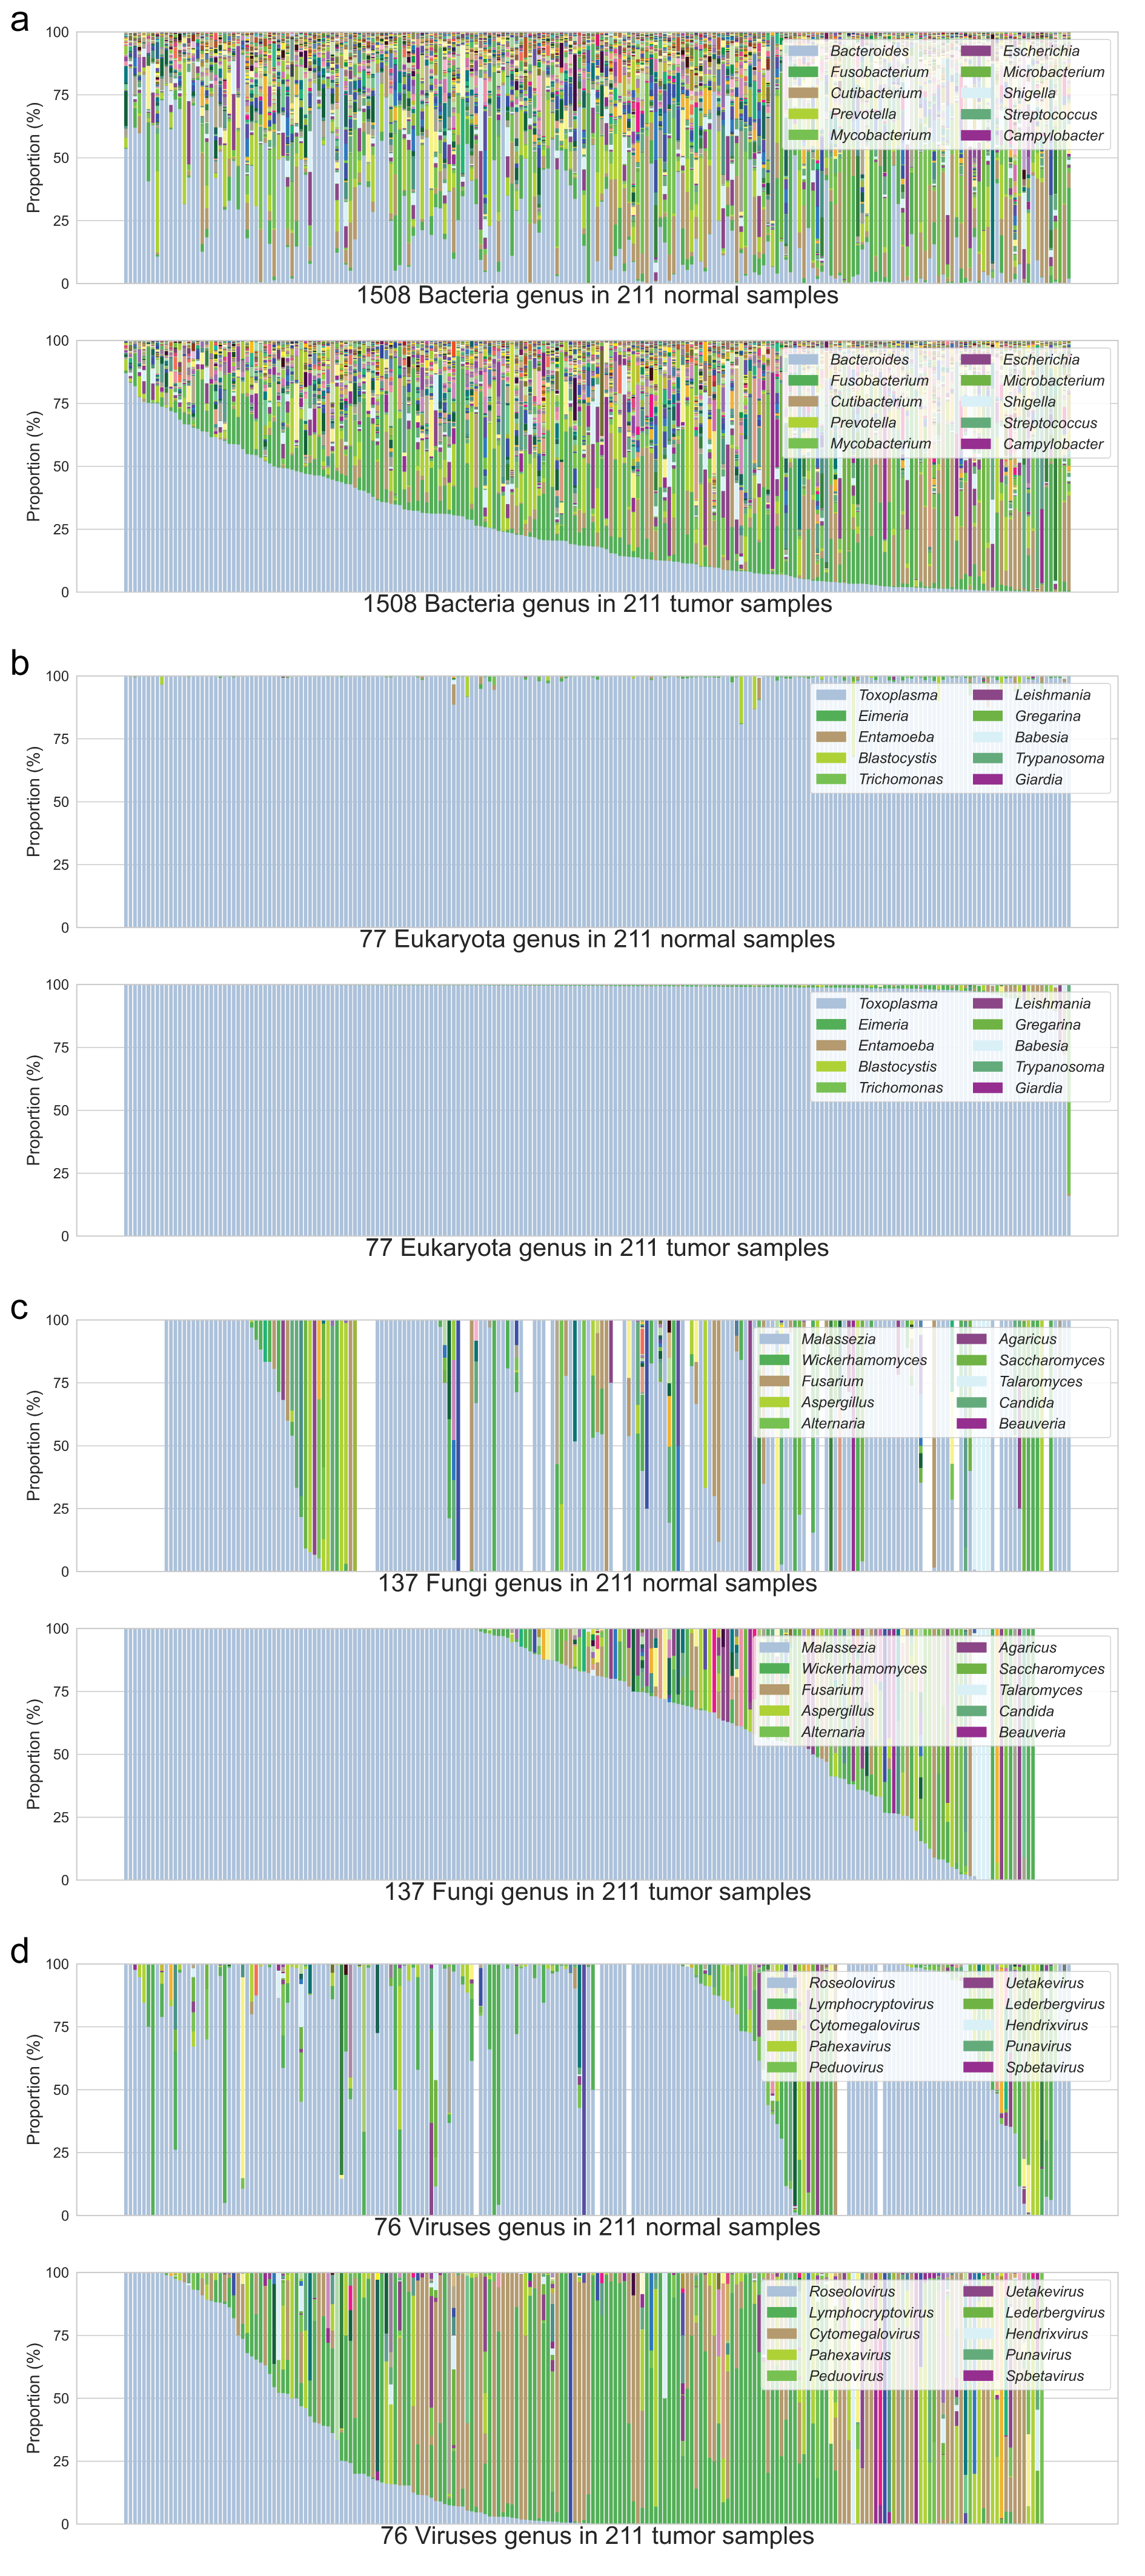
\includegraphics[width=0.6 \linewidth]{Figures/CRC/Figure_01.png}
                \caption[Gut microbiome compositions in genus level]{\textbf{Gut microbiome compositions in genus level.}\\
                    Taxa were sorted from the most prevalent taxon to the least prevalent taxon. CRC patients were sorted by the most prevalent taxon in descending order. \textbf{(a)} Bacteria kingdom \textbf{(b)} Eukaryota kingdom \textbf{(c)} Fungi kingdom \textbf{(d)} Viruses kingdom}
                \label{fig:CRC-composition}
            \end{figure}
            \clearpage

            \begin{figure}[p]
                \centering
                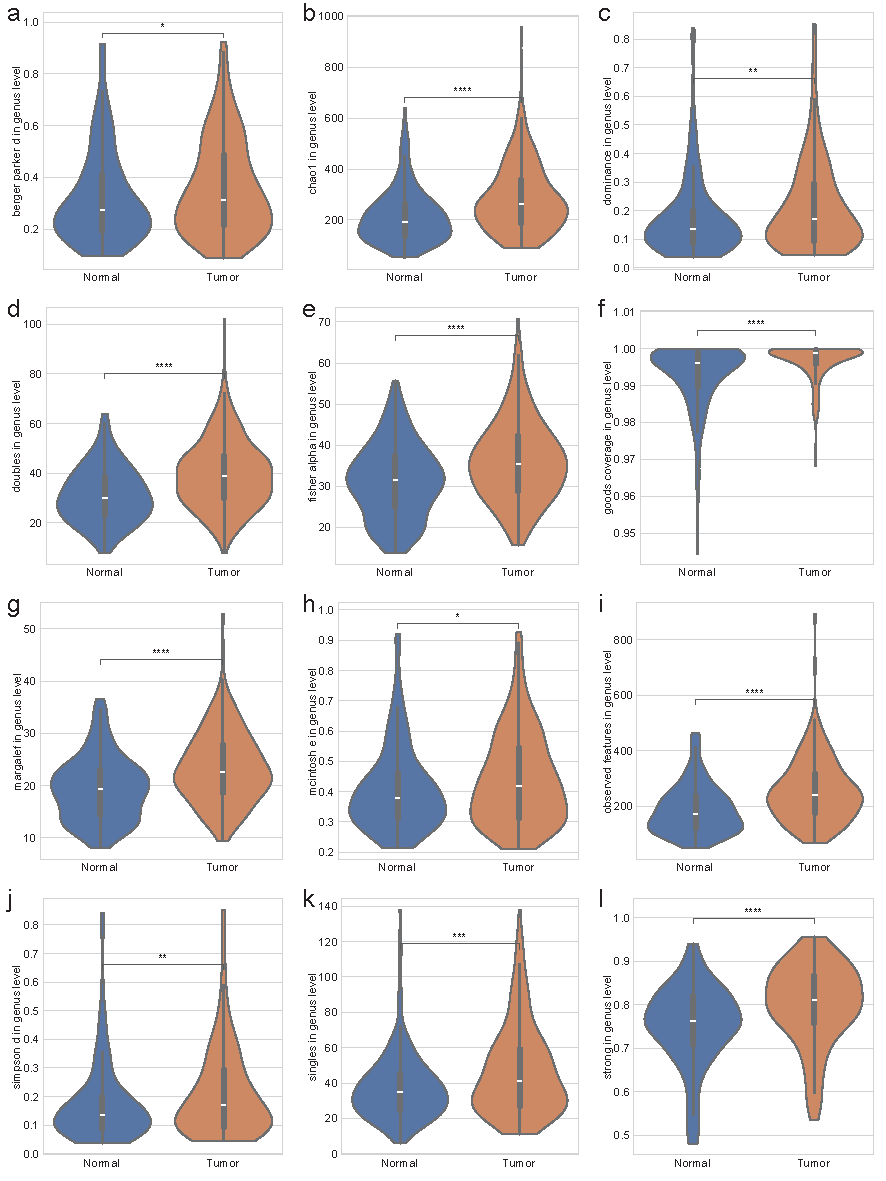
\includegraphics[width=\linewidth]{Figures/CRC/Figure_02.pdf}
                \caption[Alpha-diversity indices in genus level]{\textbf{Alpha-diversity indices in genus level.}\\
                    \textbf{(a)} Berger-Parker $d$ \textbf{(b)} Chao1 \textbf{(c)} Dominance \textbf{(d)} Doubles \textbf{(e)} Fisher $\alpha$ \textbf{(f)} Good's coverage \textbf{(g)} Margalef \textbf{(h)} Mcintosh \textbf{(i)} Observed features \textbf{(j)} Simpson $d$ \textbf{(k)} Singles \textbf{(l)} Strong. MWU test: $p < 0.05$ (*), $p < 0.01$ (**), $p < 0.001$ (***), and $p < 0.0001$ (****)}
                \label{fig:CRC-alpha}
            \end{figure}
            \clearpage

            \begin{figure}[p]
                \centering
                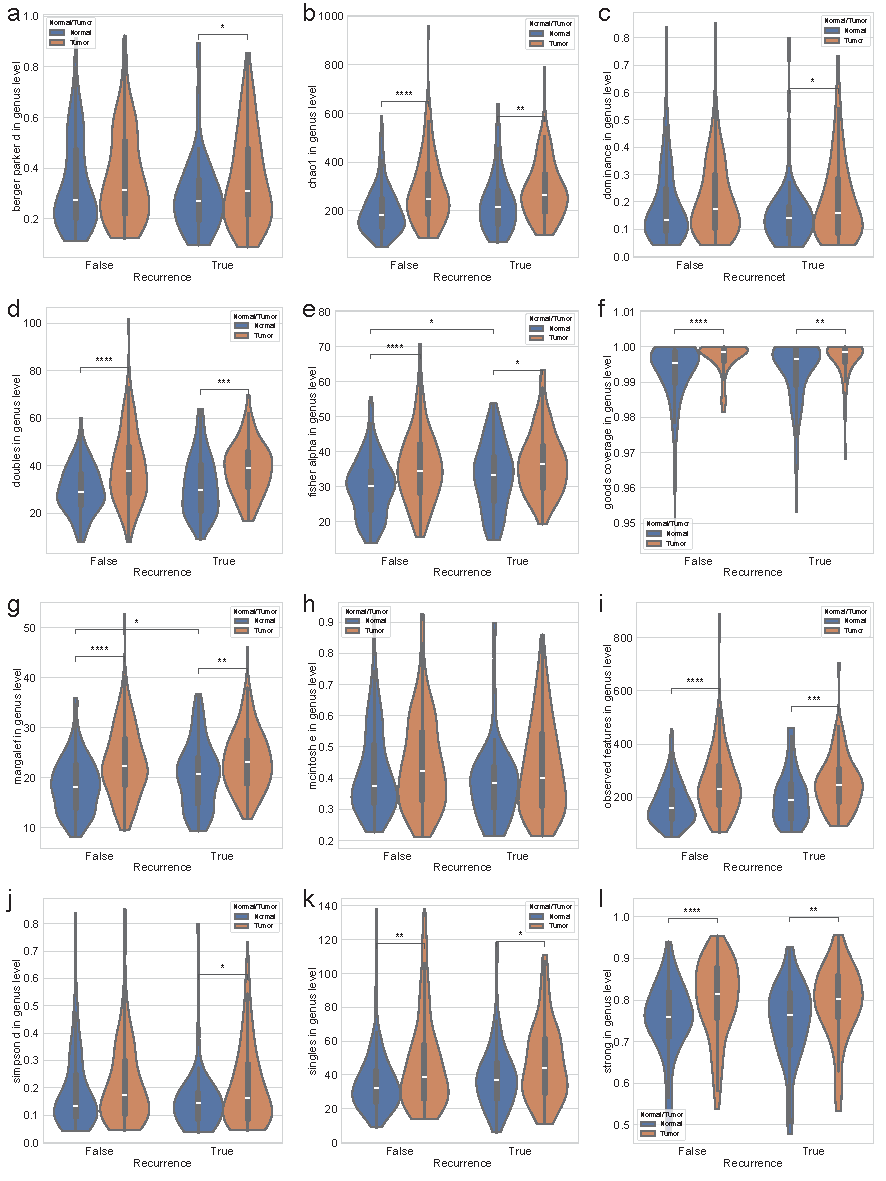
\includegraphics[width=\linewidth]{Figures/CRC/Figure_03.pdf}
                \caption[Alpha-diversity indices with recurrence in genus level]{\textbf{Alpha-diversity indices with recurrence in genus level.}\\
                    \textbf{(a)} Berger-Parker $d$ \textbf{(b)} Chao1 \textbf{(c)} Dominance \textbf{(d)} Doubles \textbf{(e)} Fisher $\alpha$ \textbf{(f)} Good's coverage \textbf{(g)} Margalef \textbf{(h)} Mcintosh \textbf{(i)} Observed features \textbf{(j)} Simpson $d$ \textbf{(k)} Singles \textbf{(l)} Strong. MWU test: $p < 0.05$ (*), $p < 0.01$ (**), $p < 0.001$ (***), and $p < 0.0001$ (****)}
                \label{fig:CRC-alpha-recurrence}
            \end{figure}
            \clearpage

            \begin{figure}[p]
                \centering
                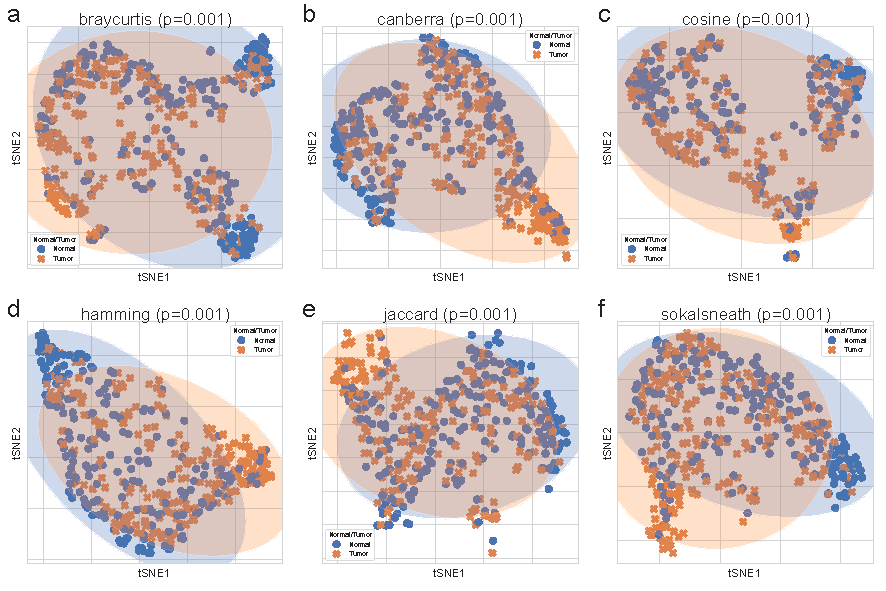
\includegraphics[width=\linewidth]{Figures/CRC/Figure_04.pdf}
                \caption[Alpha-diversity indices with OS in genus level]{\textbf{Alpha-diversity indices with OS in genus level.}\\
                    \textbf{(a)} Berger-Parker $d$ \textbf{(b)} Chao1 \textbf{(c)} Dominance \textbf{(d)} Doubles \textbf{(e)} Fisher $\alpha$ \textbf{(f)} Good's coverage \textbf{(g)} Margalef \textbf{(h)} Mcintosh \textbf{(i)} Observed features \textbf{(j)} Simpson $d$ \textbf{(k)} Singles \textbf{(l)} Strong. Statistical significance was calculated by the Spearman correlation.}
                \label{fig:CRC-alpha-OS}
            \end{figure}
            \clearpage

            \begin{figure}[p]
                \centering
                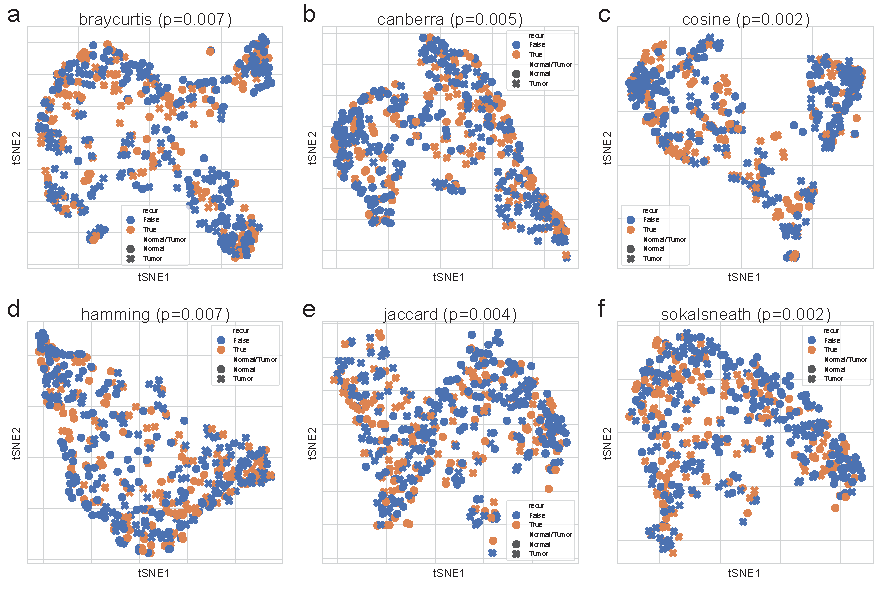
\includegraphics[width=\linewidth]{Figures/CRC/Figure_05.pdf}
                \caption[Beta-diversity indices in genus level]{\textbf{Beta-diversity indices in genus level}.\\
                    Beta-diversity indices were visualized using a tSNE-transformed plot. The confidence ellipses are shown to display the distribution of each sub-group (Normal or Tumor). \textbf{(a)} Bray-Curtis \textbf{(b)} Canberra \textbf{(c)} Cosine \textbf{(d)} Hamming \textbf{(e)} Jaccard \textbf{(f)} Sokal-Sneath. Statistical significance were determined by PERMANOVA test.}
                \label{fig:CRC-beta}
            \end{figure}
            \clearpage

            \begin{figure}[p]
                \centering
                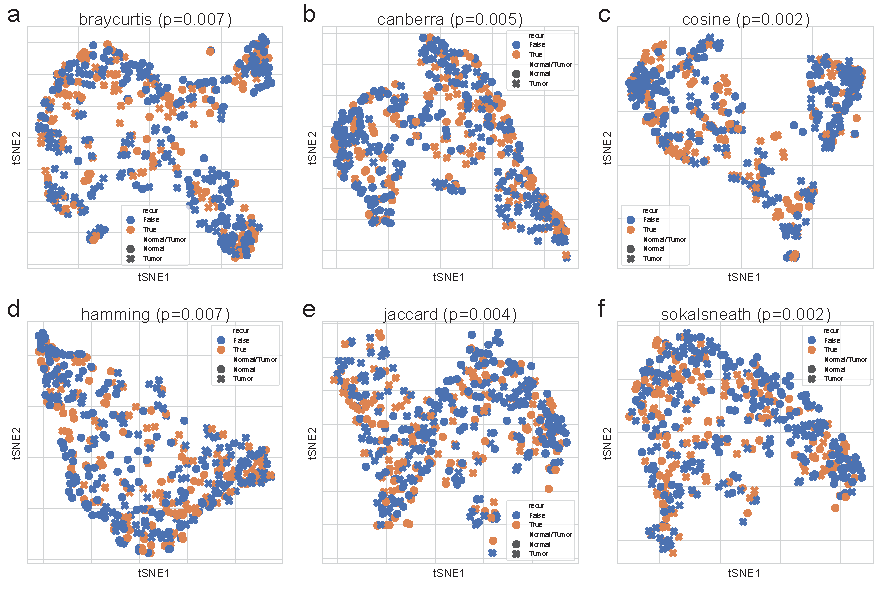
\includegraphics[width=\linewidth]{Figures/CRC/Figure_06.pdf}
                \caption[Beta-diversity indices with recurrence in genus level]{\textbf{Beta-diversity indices with recurrence in genus level}.\\
                    Beta-diversity indices were visualized using a tSNE-transformed plot. \textbf{(a)} Bray-Curtis \textbf{(b)} Canberra \textbf{(c)} Cosine \textbf{(d)} Hamming \textbf{(e)} Jaccard \textbf{(f)} Sokal-Sneath. Statistical significance were determined by PERMANOVA test.}
                \label{fig:CRC-beta-recurrence}
            \end{figure}
            \clearpage

            \begin{figure}[p]
                \centering
                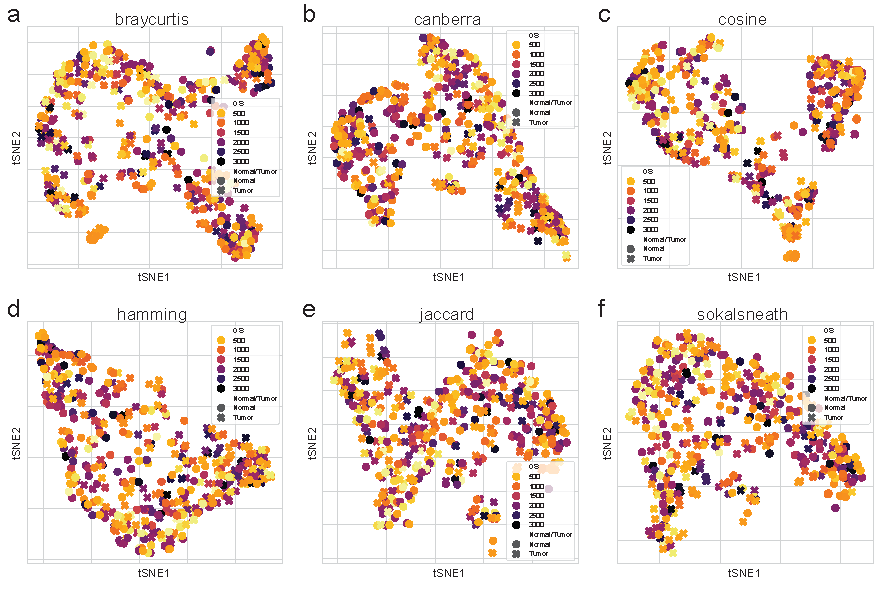
\includegraphics[width=\linewidth]{Figures/CRC/Figure_07.pdf}
                \caption[Beta-diversity indices with recurrence in genus level]{\textbf{Beta-diversity indices with OS in genus level.}\\
                    Beta-diversity indices were visualized using a tSNE-transformed plot. {(a)} Bray-Curtis \textbf{(b)} Canberra \textbf{(c)} Cosine \textbf{(d)} Hamming \textbf{(e)} Jaccard \textbf{(f)} Sokal-Sneath.}
                \label{fig:CRC-beta-OS}
            \end{figure}
            \clearpage

            \begin{figure}[p]
                \centering
                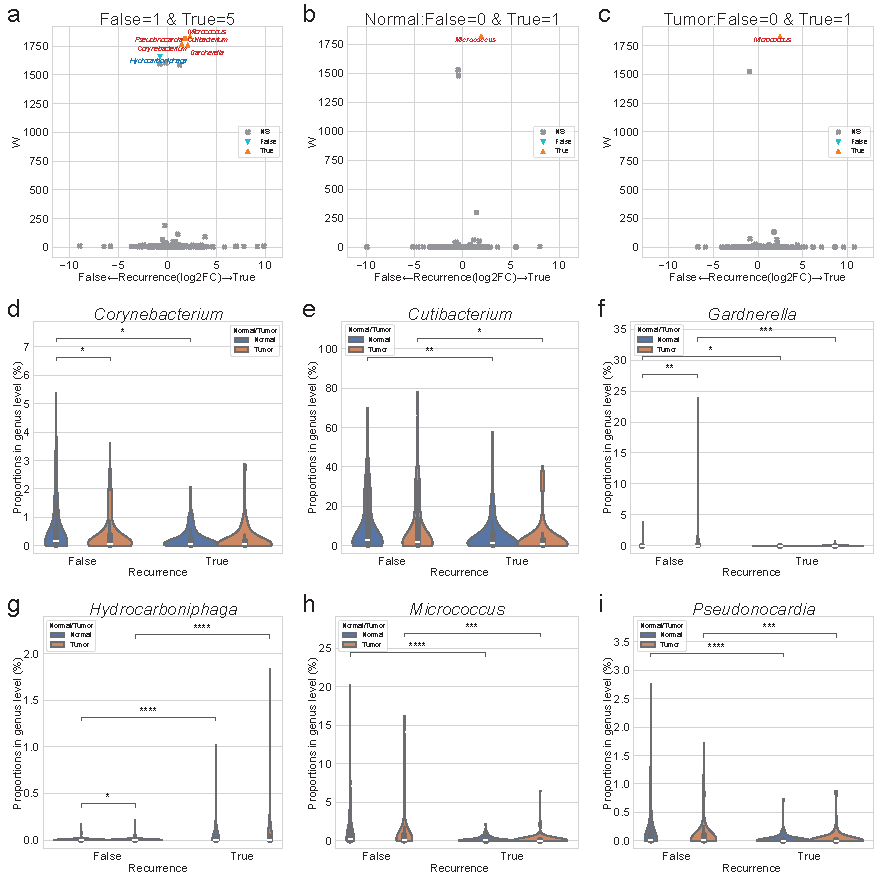
\includegraphics[width=\linewidth]{Figures/CRC/Figure_08.pdf}
                \caption[DAT with recurrence in genus level]{\textbf{DAT with recurrence in genus level.}\\
                    \textbf{(a-c)} Volcano plots with recurrence. $x$-axis indicates $\log_2 (\textrm{Fold Change})$ on recurrence, and $y$-axis indicates ANCOM significance (W). \textbf{(a)} Total \textbf{(b)} Normal samples \textbf{(c)} Tumor samples. \textbf{(d-i)} Violin plots of each taxon proportion with recurrence. \textbf{(d)} \textit{Corynebacterium} genus \textbf{(e)} \textit{Cutibacterium} genus \textbf{(f)} \textit{Gardnerella} genus \textbf{(g)} \textit{Hydrocarboniphaga} genus \textbf{(h)} \textit{Micrococcus} genus \textbf{(i)} \textit{Pseudocardia} genus. MWU test: $p < 0.05$ (*), $p < 0.01$ (**), $p < 0.001$ (***), and $p < 0.0001$ (****)}
                \label{fig:CRC-DAT-recurrence}
            \end{figure}
            \clearpage

            \begin{figure}[p]
                \centering
                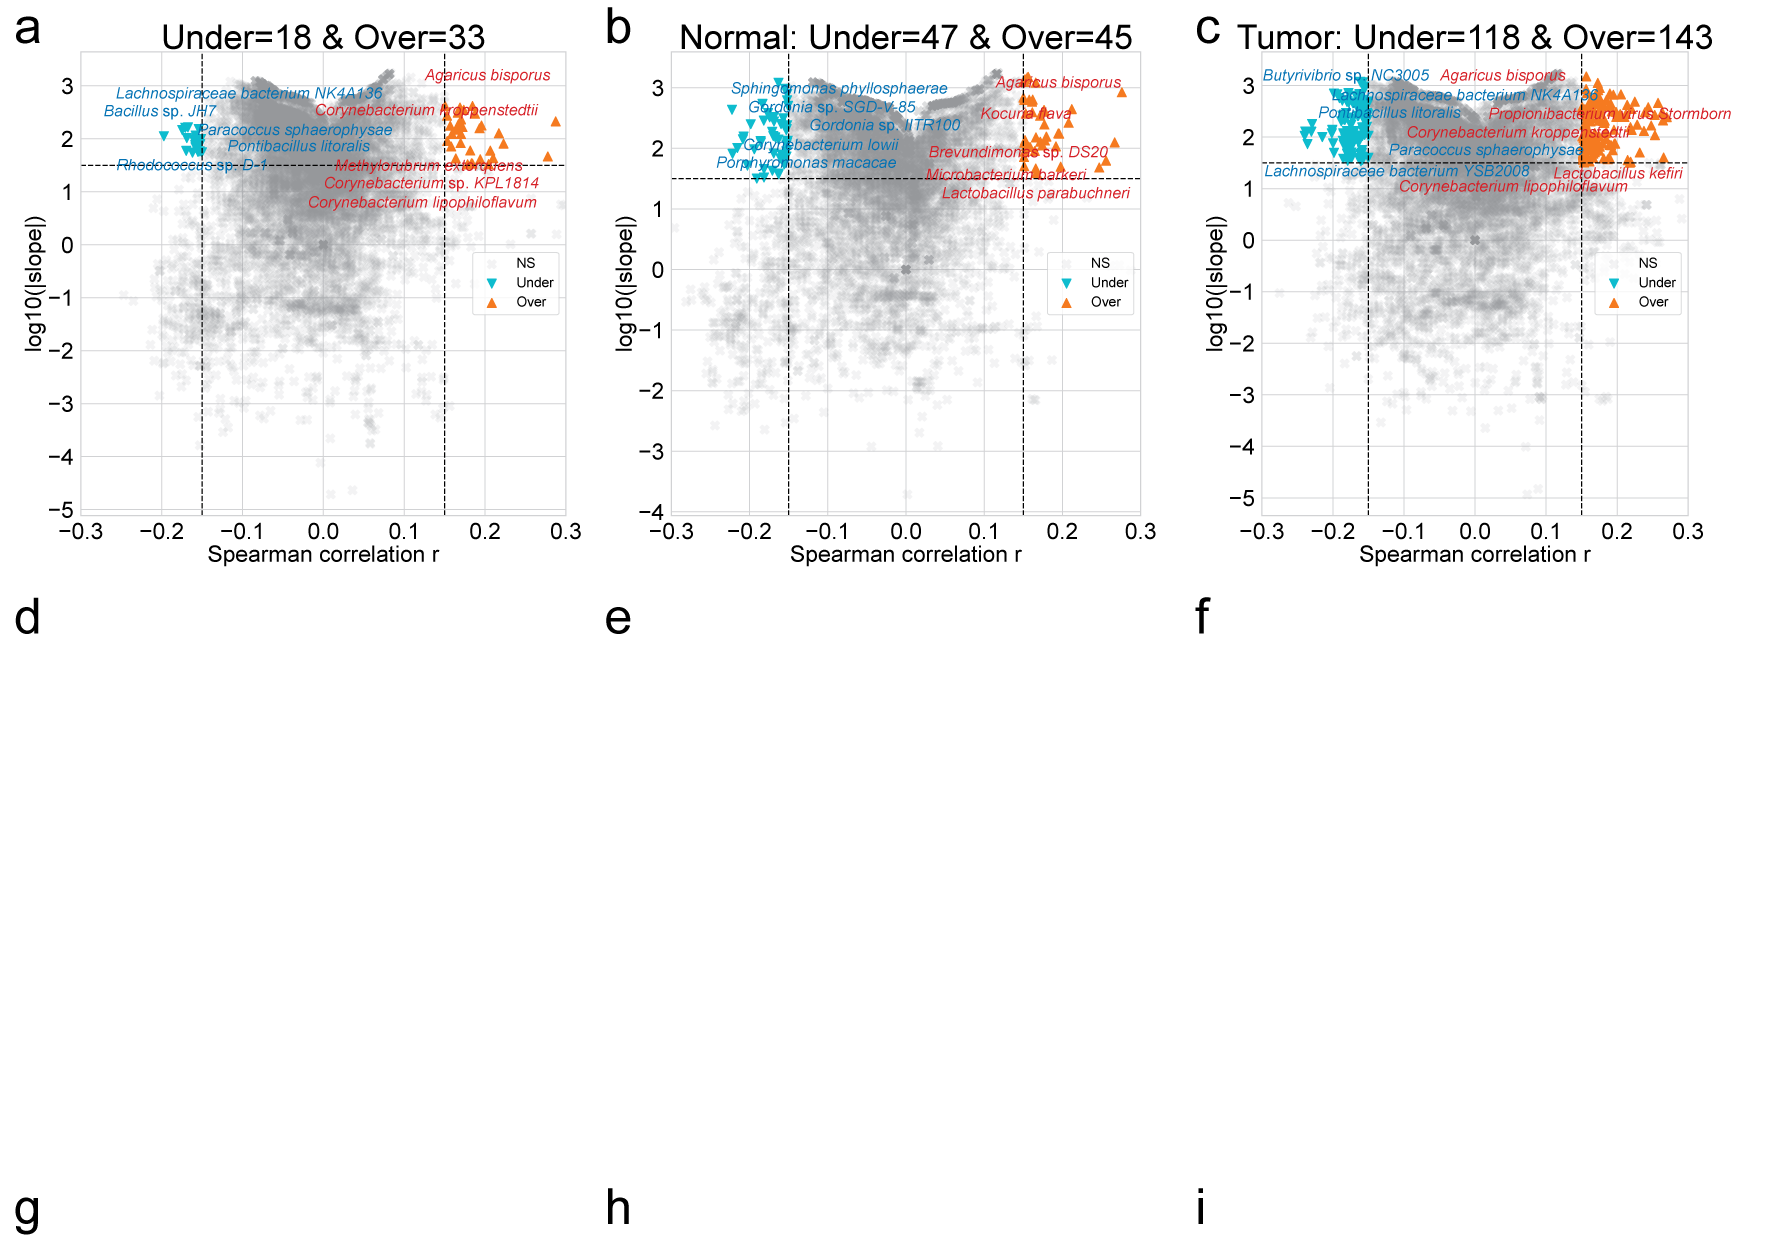
\includegraphics[width=0.9 \linewidth]{Figures/CRC/Figure_09.pdf}
                \caption[DAT with OS in genus level]{\textbf{DAT with OS in genus level.}\\
                    \textbf{(a-c)} Volcano plots with OS. $x$-axis indicates Spearman correlation coefficient ($r$), and $y$-axis indicates $\log_{10} (| \textrm{slope} |)$. \textbf{(a)} Total \textbf{(b)} Normal samples \textbf{(c)} Tumor samples. \textbf{(d-l)} Scatter plots of each taxon proportion with OS. \textbf{(d)} \textit{Alcaligenes} genus \textbf{(e)} \textit{Catabacter} genus \textbf{(f)} \textit{Enorma} genus \textbf{(g)} \textit{Kineothrix} genus \textbf{(h)} \textit{Lampropedia} genus \textbf{(i)} \textit{Methylorubrum} genus \textbf{(j)} \textit{Rodentibacter} genus \textbf{(k)} \textit{Turicibacter} genus \textbf{(l)} \textit{Weeksella} genus. Statistical significance were calculated with Spearman correlation ($r$ and $p$).}
                \label{fig:CRC-DAT-OS}
            \end{figure}
            \clearpage

            \begin{figure}[p]
                \centering
                \caption{\textbf{ML prediction.}}
            \end{figure}
            \clearpage
        \clearpage

        \subsection{Discussion}
        \clearpage
    \newpage

    \section{Conclusion}
        \label{section:conclusion}
        In conclusion, the research described in this doctoral dissertation was conducted to identify significant ...

        In the section \ref{section:PTB}, I show that
        \newpage

% Reference
    \addcontentsline{toc}{section}{References}
    \bibliographystyle{apacite}
    \bibliography{references.bib}
    \clearpage

% Acknowledgements
    \addcontentsline{toc}{section}{Acknowledgments}
    \section*{\hfill \Large Acknowledgments \hfill}
        I would like to disclose my earnest appreciation for my advisor, Professor \textbf{Semin Lee}, who provided solicitous supervision and cherished opportunities throughout the course of my research. His advice and consultation encouraged me to become as a researcher and to receive all humility and gentleness. I am also grateful to all of my committee members, Professor \textbf{Taejoon Kwon}, Professor \textbf{Eunhee Kim}, Professor \textbf{Kyemyung Park}, and Professor \textbf{Min Hyuk Lim}, for their meaningful mentions and suggestions.

        I extend my deepest gratitude to my Lord, \textbf{the Flying Spaghetti Monster}, His Noodly Appendage has guided me through the twist and turns of this academic journey. His presence, ever comforting and mysterious, has been a source of strength and humor during both highs and lows. In moments of doubt, I found solace in the belief that you were there, gently reminding me to keep faith in the process. His Holy Noodle has nourished my mind, and for that, I am truly overwhelmed. May His Holy Noodle continue to guide me in all my future endeavors. \textit{R'Amen}.

        I would like to extend my heartfelt gratitude to Professor \textbf{You Mi Hong} for her invaluable guidance and insightful advice on PTB study. Hex expertise in maternal and fetal health, along with her deep understanding of statistical and clinical interpretations, greatly contributed to refining the analytical framework of this study. Her constructive feedback and thoughtful discussions provided critical perspectives that enhanced the robustness and relevance of the research findings. I sincerely appreciate her generosity in sharing her knowledge and effort, as well as her encouragement throughout my Ph.D. journey. Her support has been instrumental in strengthening this work, and I am truly grateful for her contributions.

        I also would like to express my sincere gratitude for Professor \textbf{Jun Hyeok Lim} for his invaluable guidance and insightful advice on lung cancer study. His expertise in cancer genomics and data interpretation provided essential perspectives that greatly enriched the analytical approach of my Ph.D. journey. His constructive feedback and thoughtful discussion helped refine methodologies and enhance the scientific rigor of the research. I deeply appreciate his willingness to share his knowledge and expertise, which has been instrumental in shaping key aspects of this work. His support and encouragement have been truly inspiring, and I am grateful for the opportunity to have benefited from his mentorship.

        I would like to extend my heartfelt gratitude to my colleagues of the \textbf{Computational Biology Lab @ UNIST}, whose collaboration, friendship, brotherhood, and support have been an invaluable part of my journey. Your willingness to share insights, engage in thoughtful discussions, and offer encouragement during the challenging moments of research has significantly shaped my academic experience. The camaraderie in Computational Biology Lab made even the most demanding days more enjoyable, and I am deeply grateful for the collaborative environment we created together. I appreciate you for standing by my side throughout this Ph.D. journey.

        I would like to express my heartfelt gratitude to \textbf{my family}, whose unwavering support has been the foundation of everything I have achieved. Your love, encouragement, and belief in me have sustained me through every challenge, and I could not have come this far without you. From your words of wisdom to your patience and understanding, each of you has played a vital role in helping me navigate this journey. The strength and comfort I have drawn from our family bond have been my greatest source of resilience. Your presence, both near and far, has filled my life with warmth and motivation. I am deeply grateful for your unconditional love and for always being there when I needed you the most. Thank you for being my constant source of strength and inspiration.

        I am incredibly pleased to my friends, especially my GSHS alumni (\textbf{이망톡}), for their unwavering support and encouragement throughout this journey. The bonds we formed back in our school days have only grown stronger over the years, and I am fortunate to have had such loyal and understanding friends by my side. Your constant words of motivation, and even moments of levity during stressful times have helped keep me grounded. Whether it was a late-night conversations, a shared laugh, or a simple message of reassurance, you all have played a vital role in keeping me focused and motivated. I am relieved for the ways you celebrated each small achievement with me and how you patiently listened to my worries. The memories of our shared past provided me with comfort and a sense of stability when the road ahead felt uncertain. I could not have reached this point without the love and friendship that you all have generously given. Each of your, in your unique way, has contributed to this dissertation, even if indirectly, and for that, I am forever beholden. I look forward to continuing our friendship as we all grow in our individual paths, knowing that the support we share is something truly special.

        I would like to express my deepest recognition to \textbf{my girlfriend (expected)} for her unwavering support, patience, and companionship throughout my Ph.D. journey. Her presence has been a constant source of comfort and motivation, helping me navigate the challenges of research and writing with renewed energy. Through moments of frustration and accomplishment alike, her encouragement has reminded me of the importance of balance and perseverance. Her kindness, understanding, and belief in me have been invaluable, making even the most difficult days feel lighter. I am truly grateful for her support and for sharing this journey with me, and I look forward to all the moments we will continue to experience together.

        I would like to express my sincere gratitude to the amazing members of my animal protection groups, DRDR (\textbf{두루두루}) and UNIMALS (\textbf{유니멀스}), whose dedication and compassion have been a constant source of motivation. Your unwavering commitment to improving the lives of animals has inspired me throughout this journey. I am also thankful for the beautiful cats we have cared for, whose presence brought both joy and purpose to our allegiance. Their playful spirits and gentle companionship served as daily reminders of why we continue to fight for animal rights. The bond we share, both with each other and with the animals we protect, has enriched my life in countless ways. I appreciate you all again for your support, dedication, and for being part of this meaningful cause.

        I would like to express my deepest gratitude to \textbf{everyone} I have had the honor of meeting throughout this journey. Your kindness, encouragement, and support have carried me through both the challenging and rewarding moments of my life. Whether through a kind word, thoughtful advice, or simply being there when I needed it most, your presence has made all the difference. I am incredibly fortunate to have received such generosity and warmth from those around me, and I do not take it for granted. Every act of kindness, no matter how big or small, has been a source of strength and motivation for me. To all my friends, colleagues, mentors, and beloved ones, thank you for your unwavering support. I am truly grateful for each of you, and your kindness has left an indelible mark on my journey.

        \begin{center}
            My Lord, \textit{the Flying Spaghetti Monster},\\
            give us grace to accept with serenity the things that cannot be changed,\\
            courage to change the things that should be changed,\\
            and the wisdom to distinguish the one from the other.

            \medspace

            Glory be to \textit{the Meatball}, to \textit{the Sauce}, and to \textit{the Holy Noodle}. \\
            As it was in the beginning, is now, and ever shall be. \\
            \textit{R'Amen.}
        \end{center}

        \begin{figure*}[hp]
            \centering
            
\includegraphics[width=10 cm]{Figures/Coat of arms.pdf}
            \caption*{\textit{May your progress be evident to all}}
        \end{figure*}
    \clearpage

%%% The following page is intentionally left as blank
% White attachment form
\hbox{ }
\thispagestyle{empty}
\clearpage
\end{document}